\section{Годограф Найквиста}

В соответствии с вариантом придумаем три объекта пятого порядка с 
тремя вещественными полюсами и двумя комплексно-сопряженными. Все следующие
передаточные функции (ПФ) объектов были подобраны вручную.
 
\subsection{Объект 1}

ПФ с четырьмя неустойчивыми полюсами у разомкнутой системы и один неустойчивый полюс у замкнутой,
разомкнутая система:
\begin{equation*}
    W_1(s)=\frac{100s^4+100s^3+100s^2+100s-100}{(s-1-j)(s-1+j)(s-2)(s-3)(s+1)}
    = \frac{100s^4+100s^3+100s^2+100s-100}{s^5-6s^4+11s^3-4s^2-10s+12}.
\end{equation*}
Полюса разомкнутой и замкнутой систем можно увидеть в таблице \ref{tab:poles},
как и их изображение на комплексной плоскости на рисунке \ref{fig:obj1_pz}
вместе с нулями. Из 4 неустойчивых корней остался только 1, значит по критерию 
Найквиста разность между оборотами АФЧХ вокруг (-1; 0) против часовой стрелки и по часовой стрелке
равняется 3.

\begin{table}[h!]
    \centering
    \caption{Полюса объекта 1}
    \begin{tabular}{|c|c|}
    \hline
    \textbf{Полюса разомкнутой системы}       & \textbf{Полюса замкнутой системы}        \\ \hline
    $3.0000 + 0.0000i$ & $-92.8151 + 0.0000i$ \\ \hline
    $-1.0000 + 0.0000i$ & $-1.3498 + 0.0000i$ \\ \hline
    $2.0000 + 0.0000i$ & $-0.1663 + 1.1765i$  \\ \hline
    $1.0000 + 1.0000i$ & $-0.1663 - 1.1765i$  \\ \hline
    $1.0000 - 1.0000i$ & $0.4975 + 0.0000i$   \\ \hline
    \end{tabular}
    \label{tab:poles}
\end{table}
    

\begin{figure}[H]
    \centering
    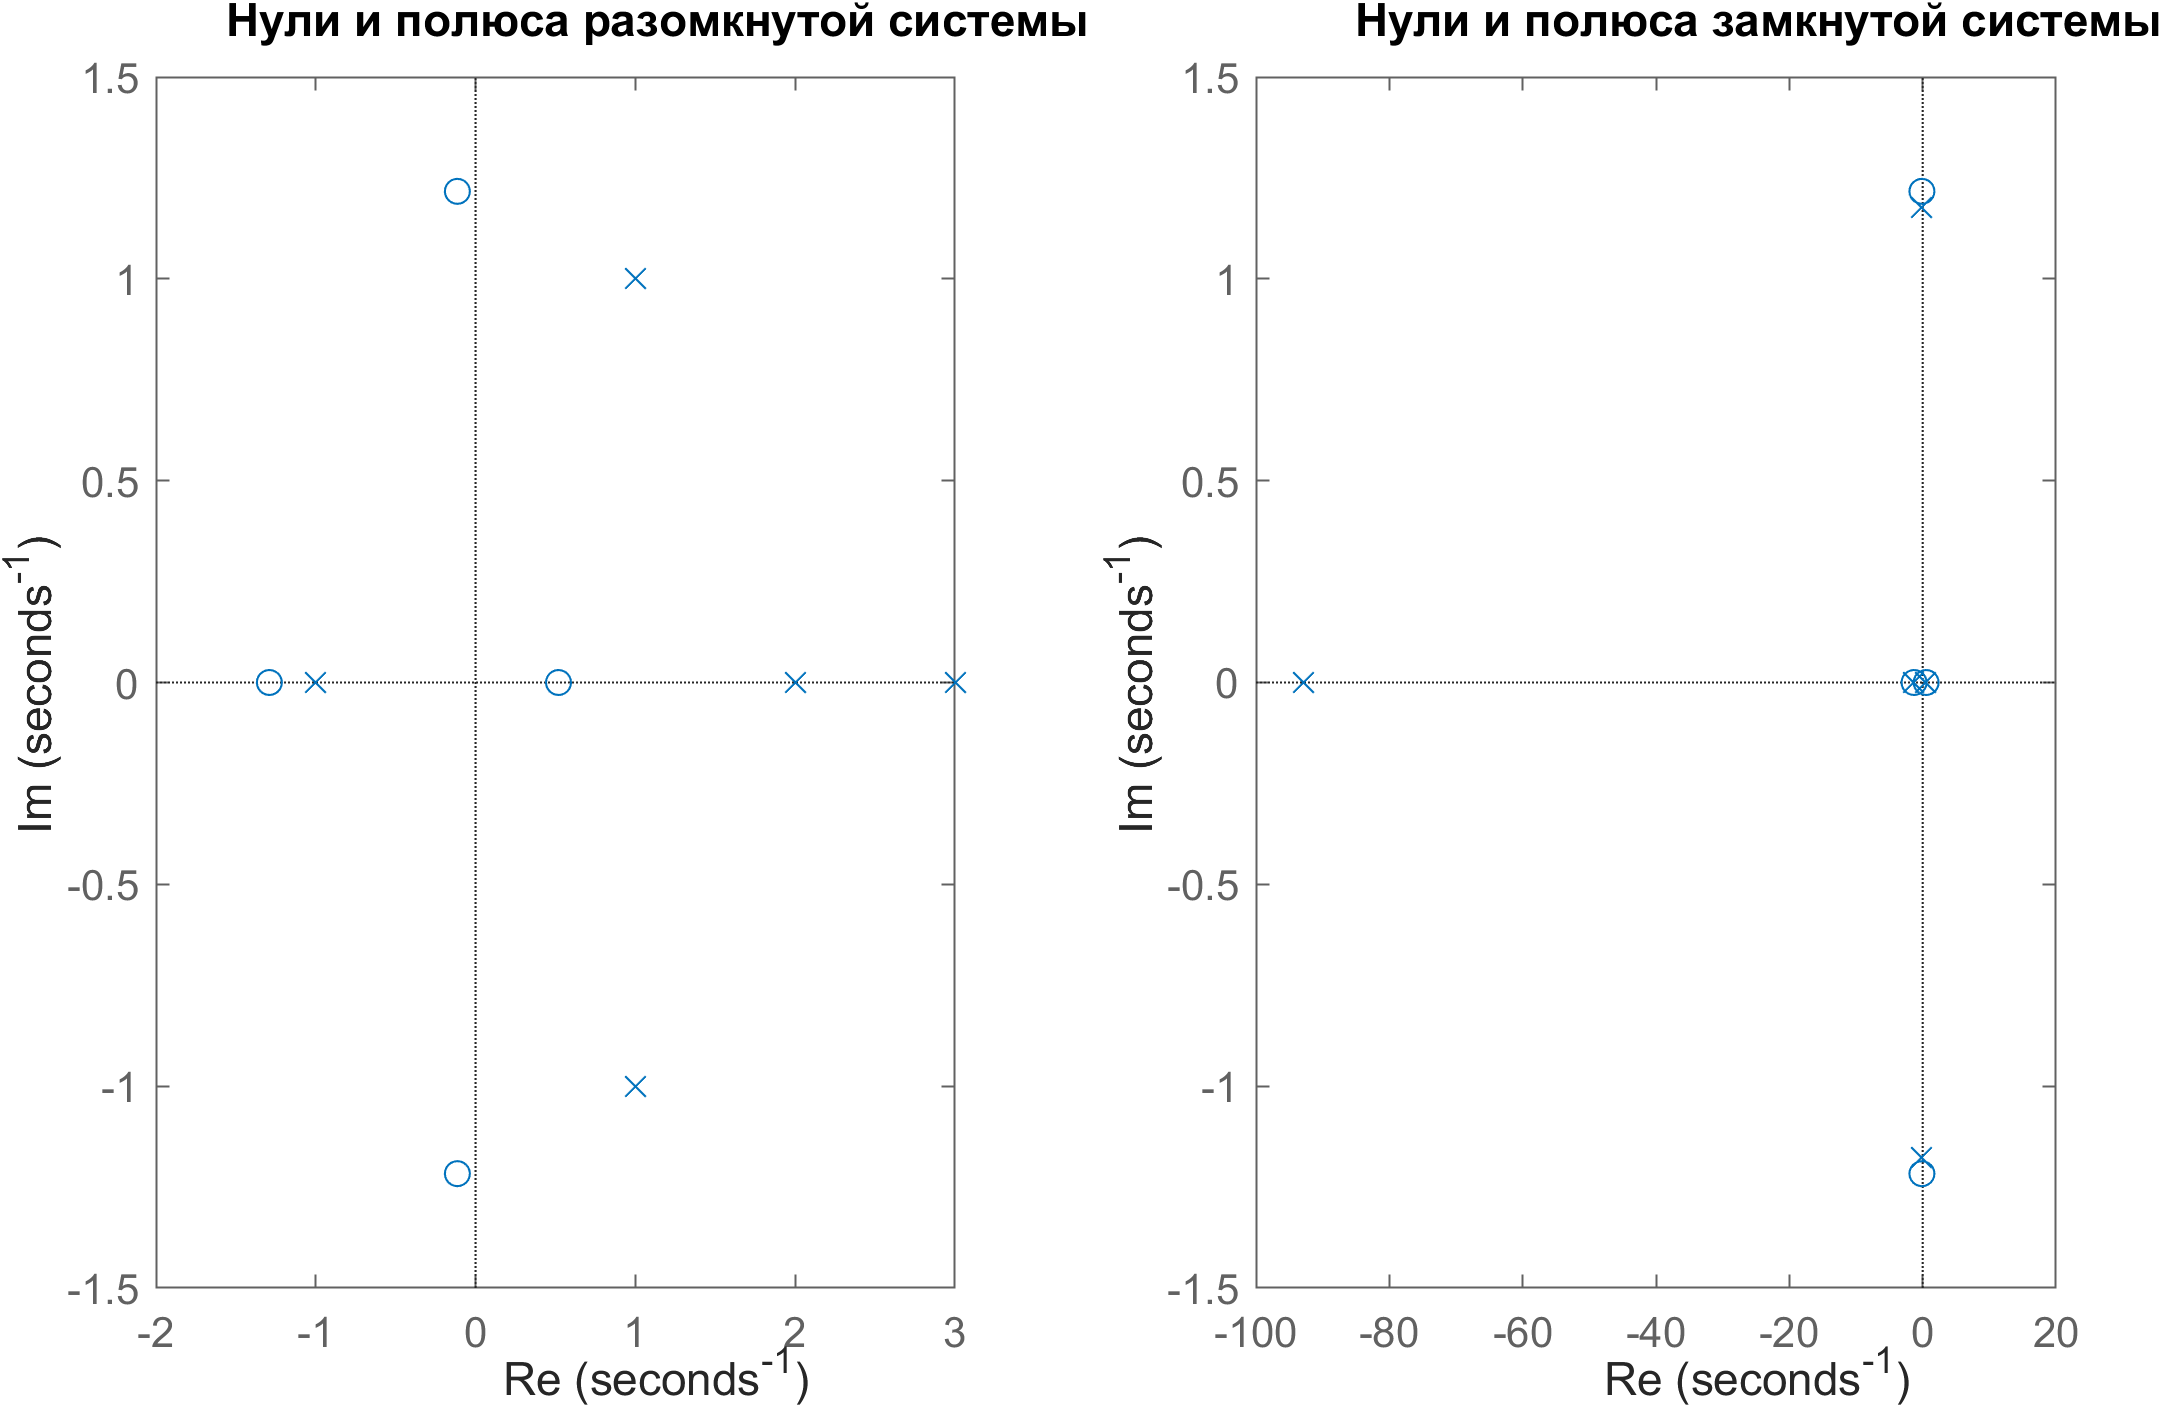
\includegraphics[width=\textwidth]{figs/task_1_obj_1_zeros_poles.png}
    \caption{Нули и полюса объекта 1}
    \label{fig:obj1_pz}
\end{figure}

\begin{figure}[H]
    \centering
    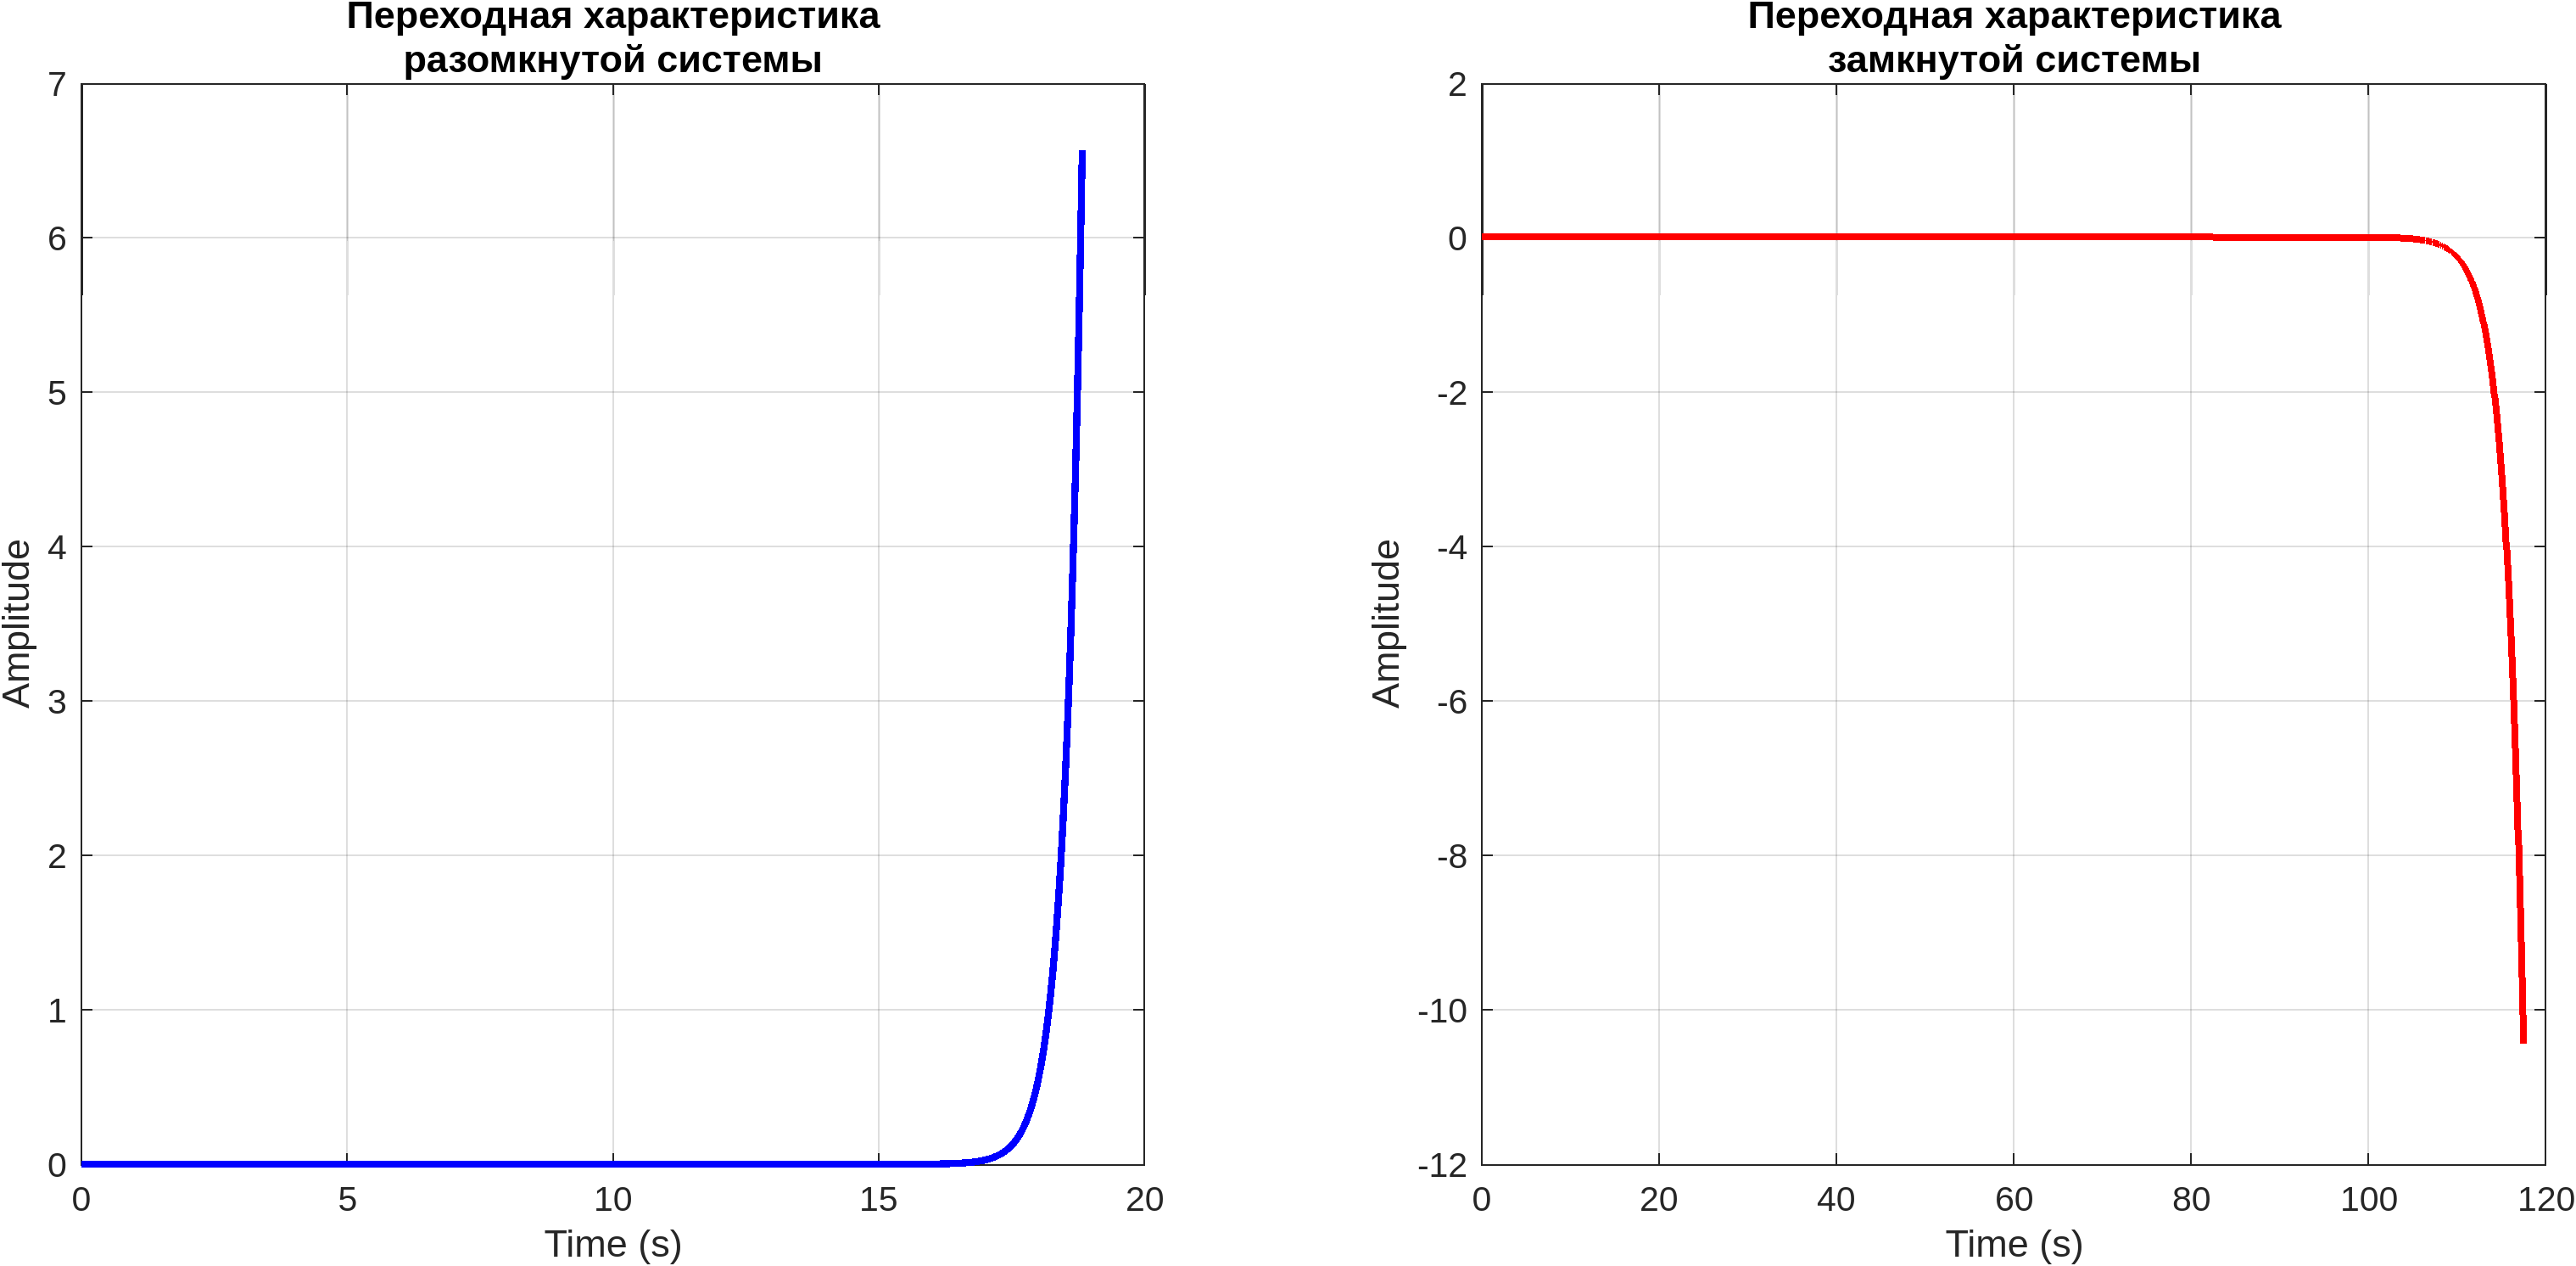
\includegraphics[width=\textwidth]{figs/task_1_obj_1_step.png}
    \caption{Переходные характеристики объекта 1}
    \label{fig:obj1_step}
\end{figure}

\begin{figure}[H]
    \centering
    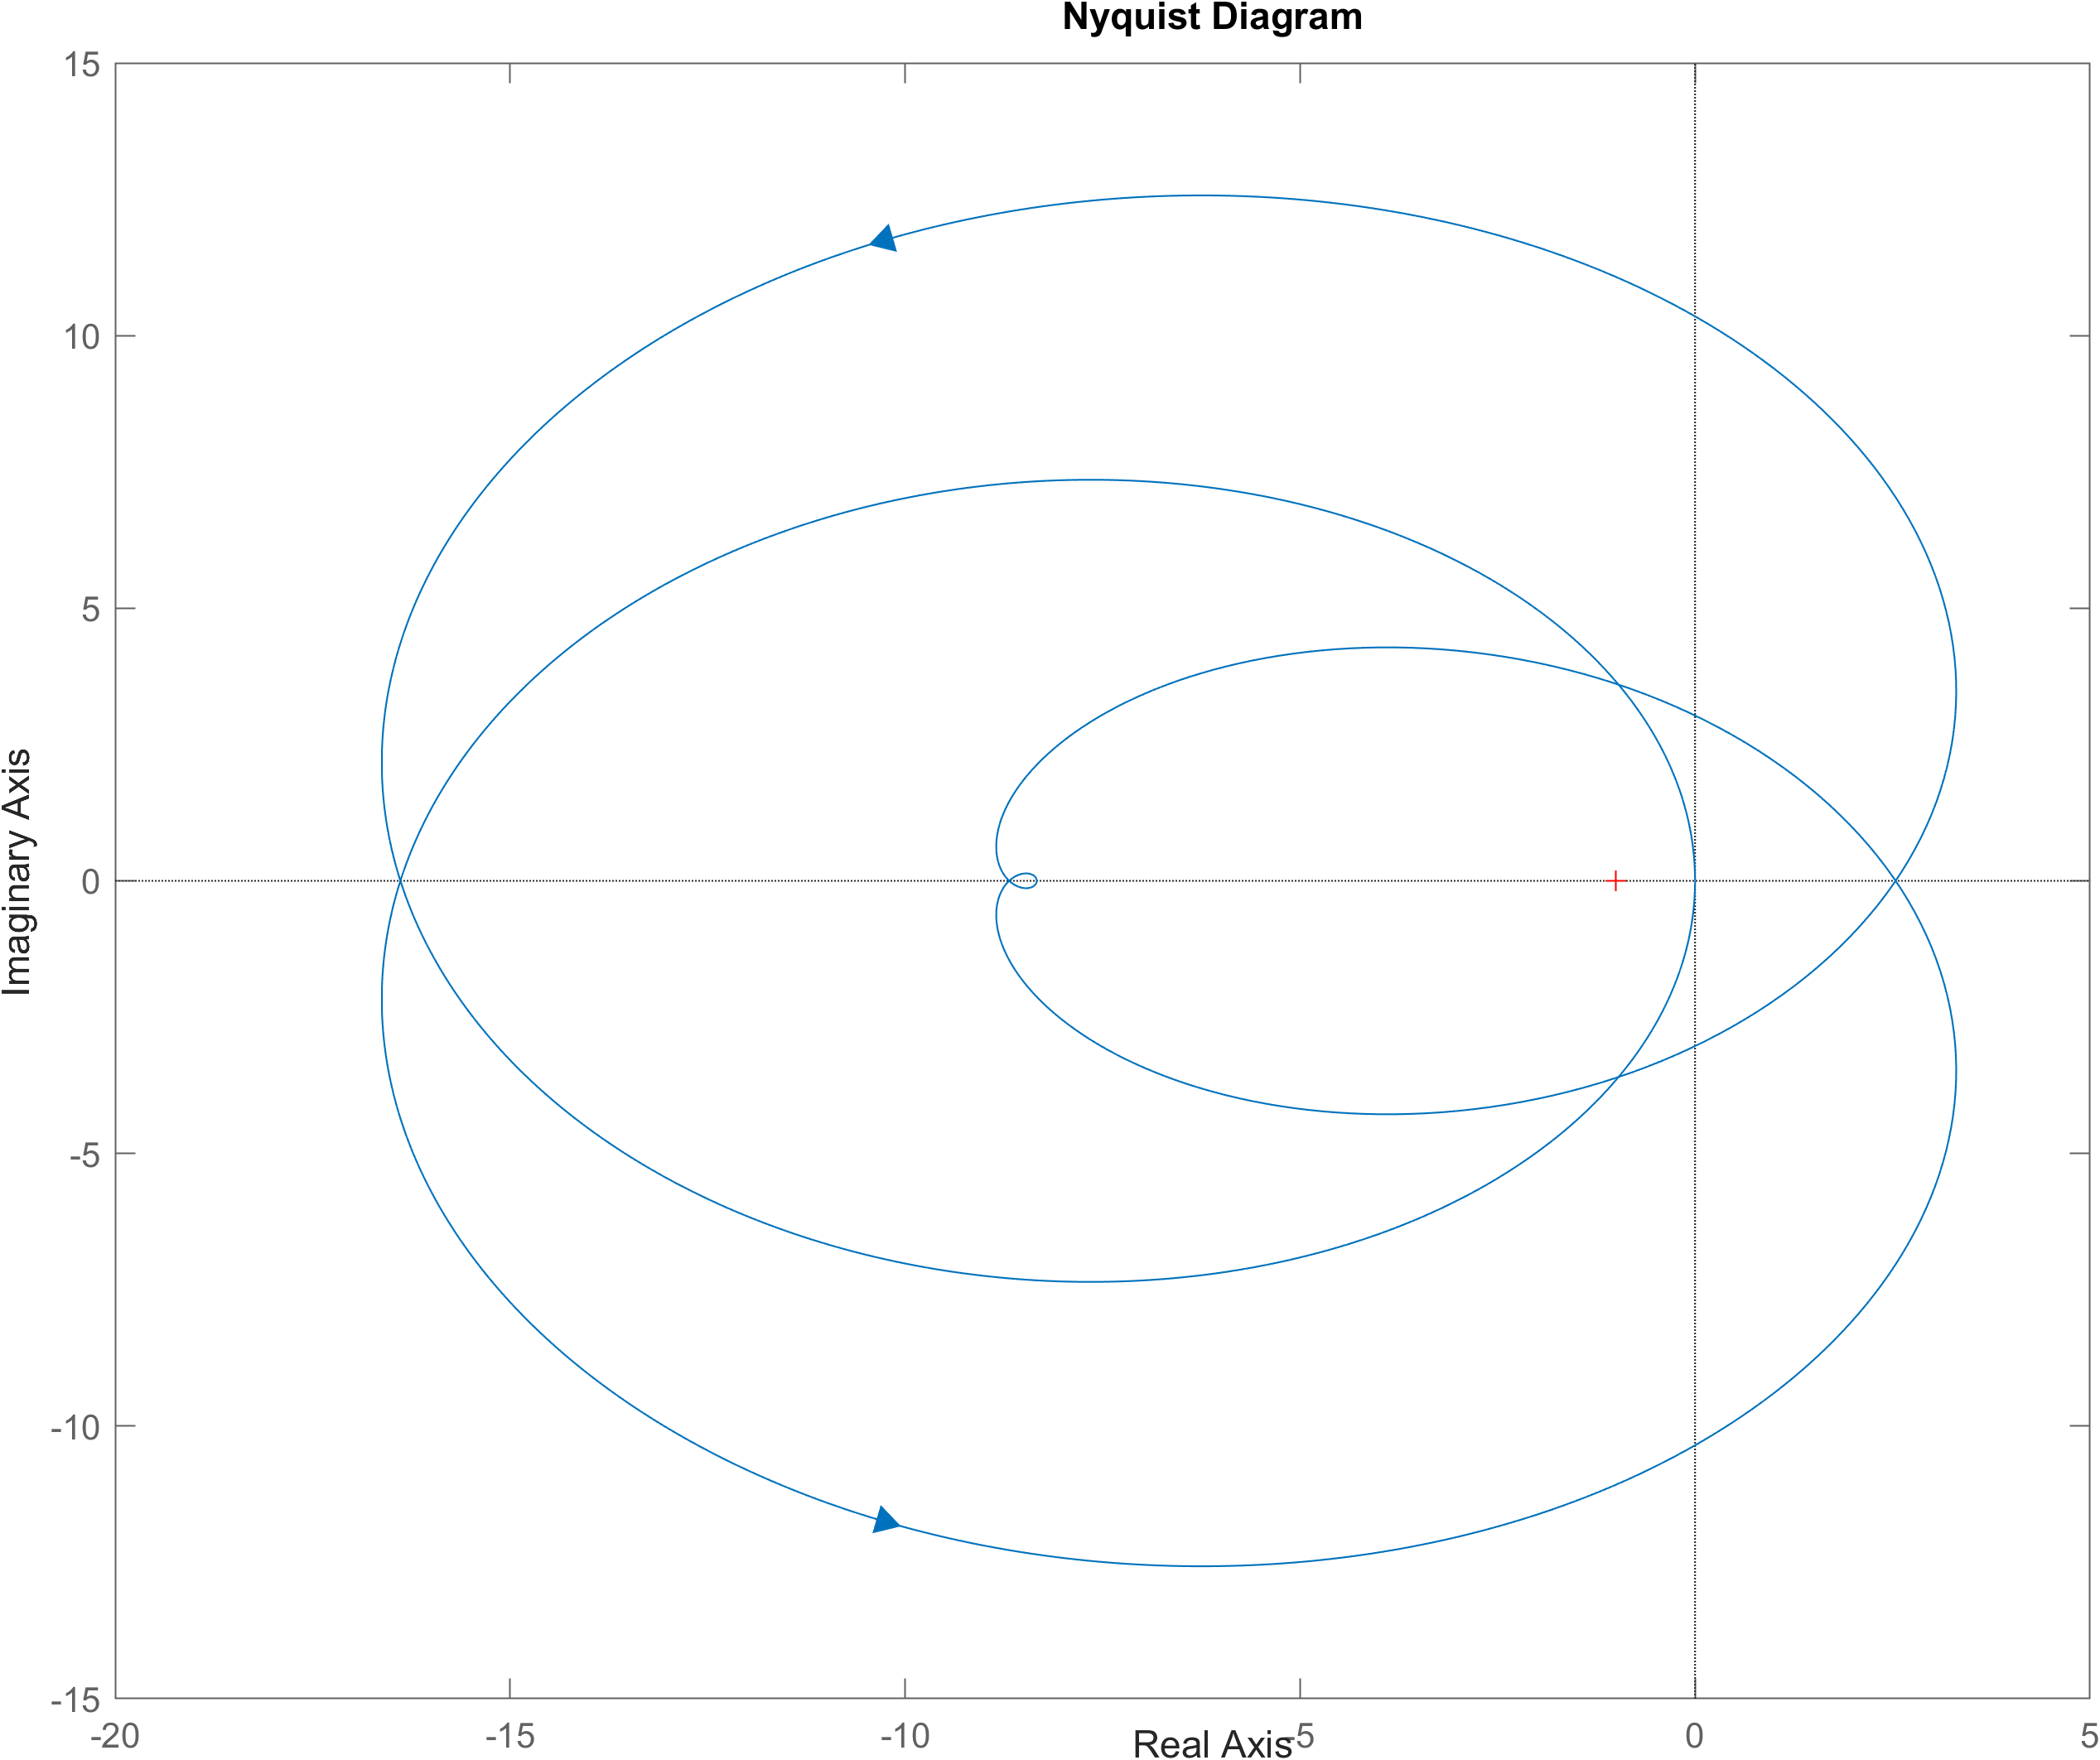
\includegraphics[width=\textwidth]{figs/task_1_obj_1_nyquist.png}
    \caption{Годограф Найквиста объекта 1}
    \label{fig:obj1_nyquist}
\end{figure}

\begin{figure}[H]
    \centering
    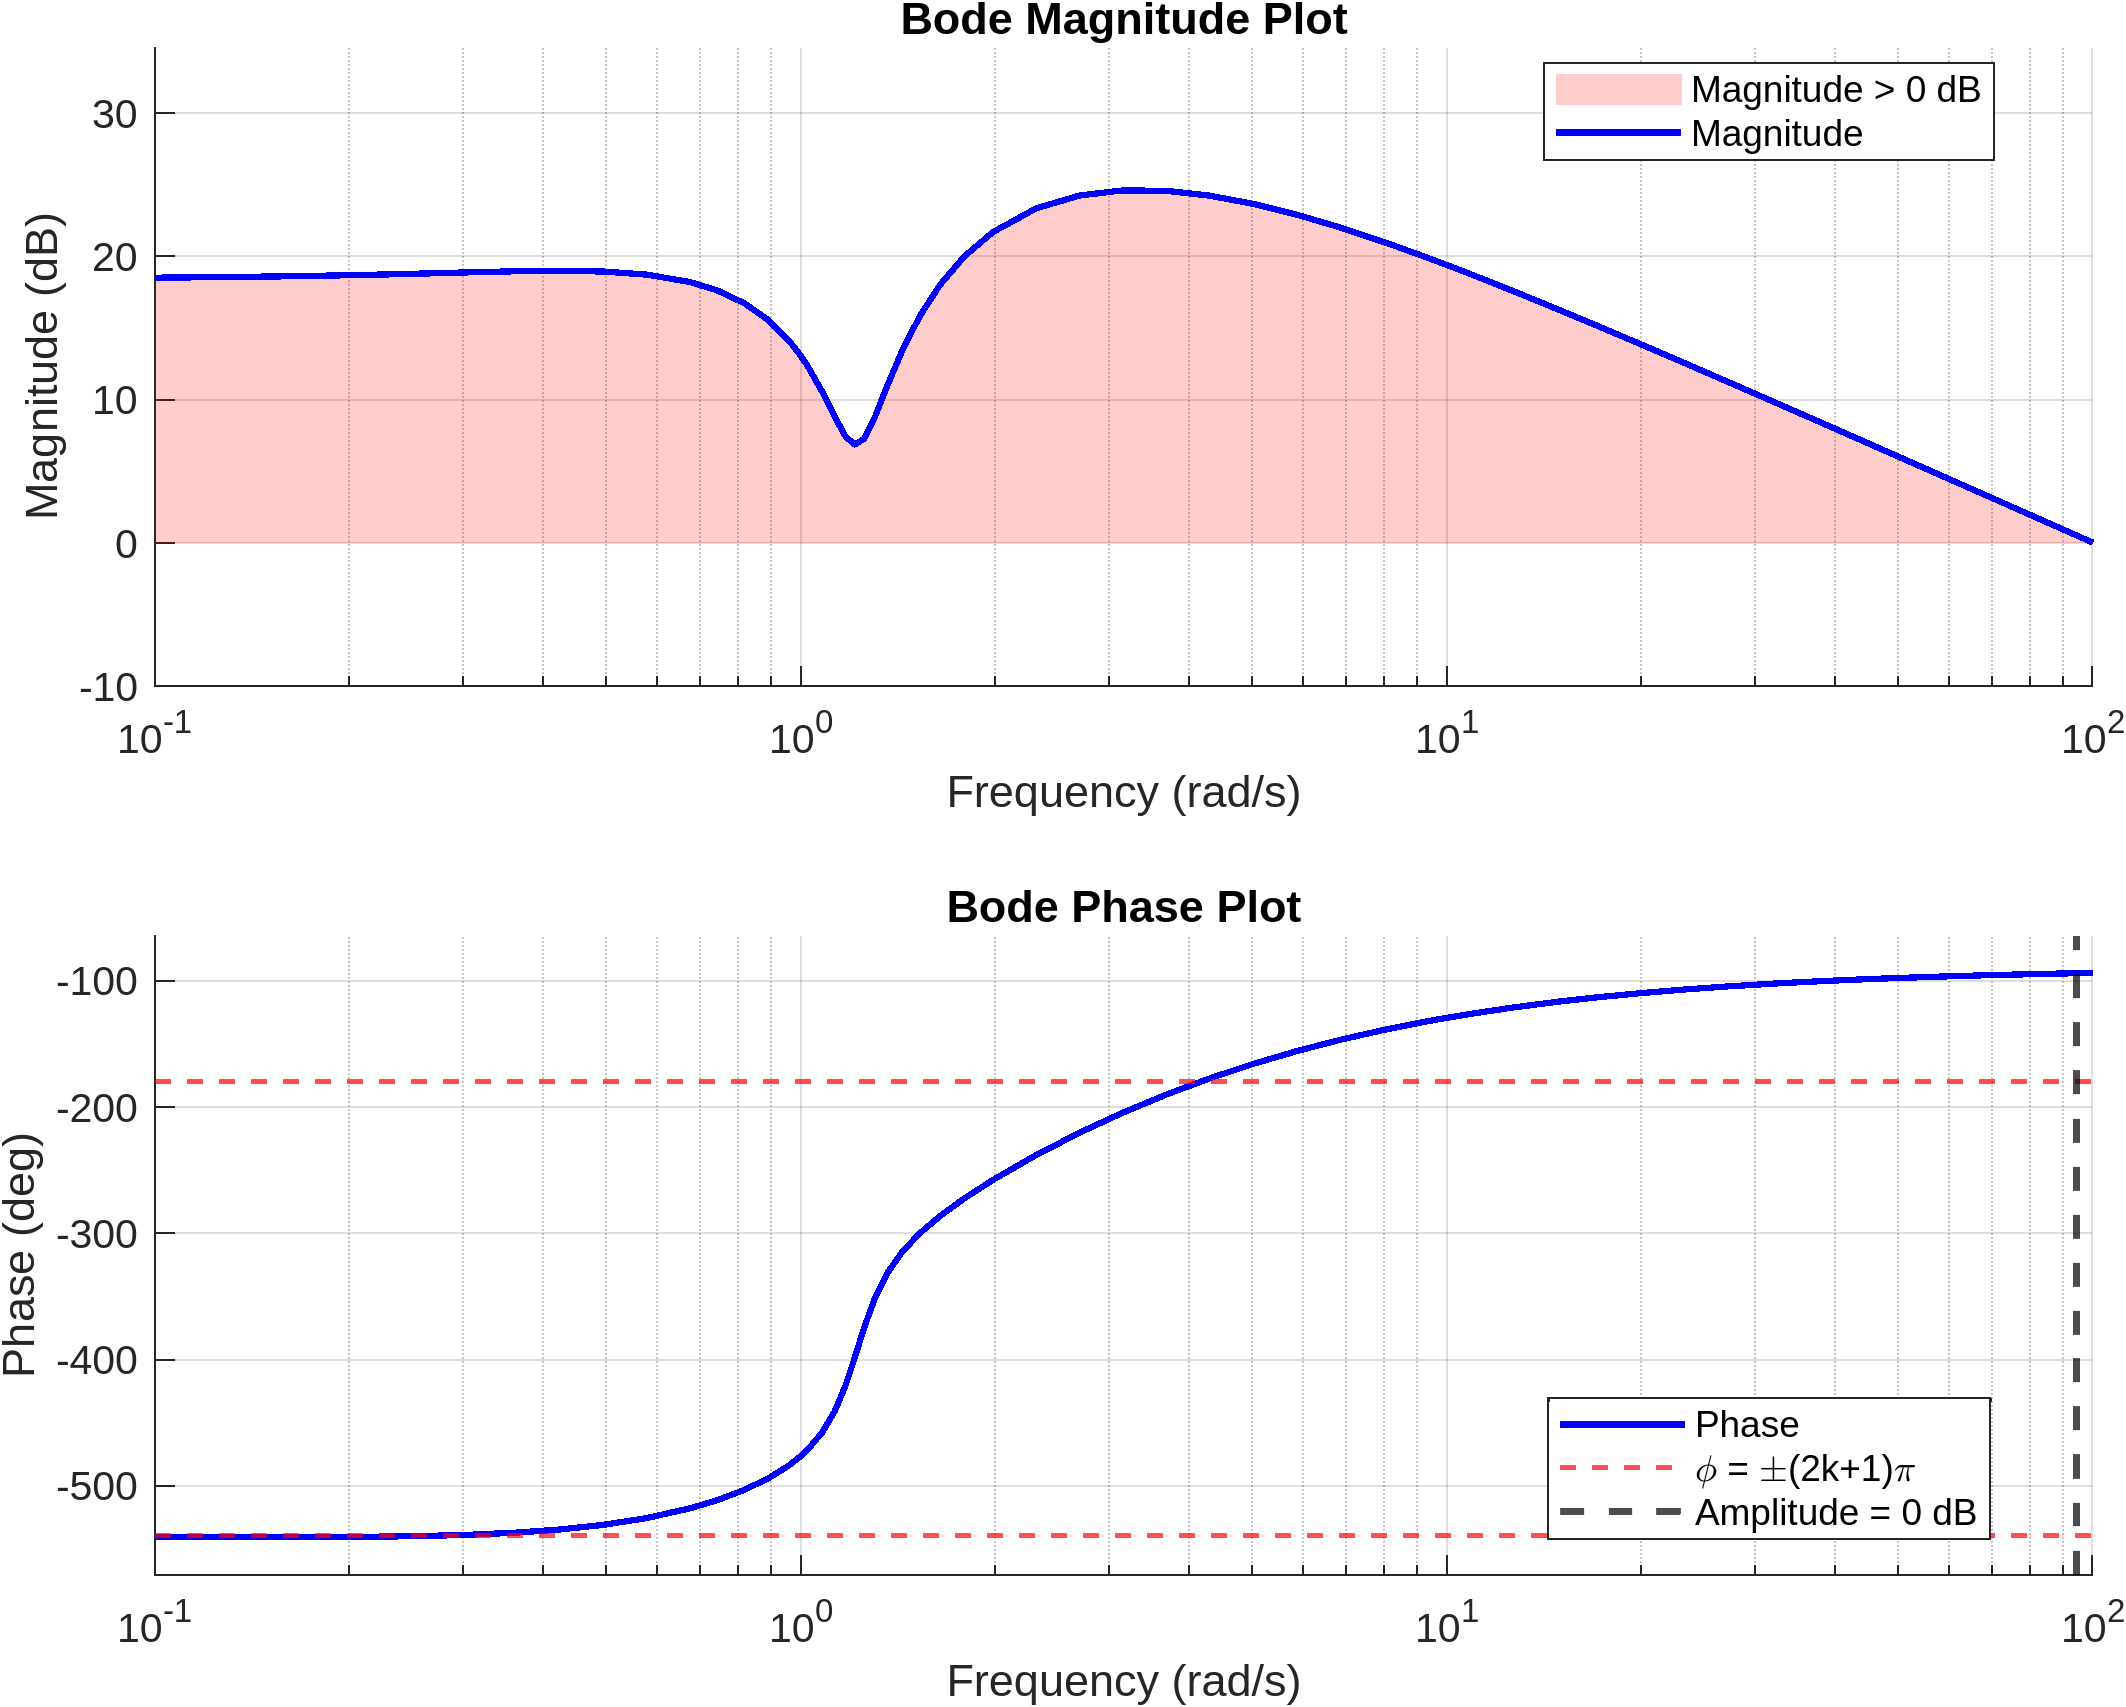
\includegraphics[width=\textwidth]{figs/task_1_obj_1_bode.png}
    \caption{ЛАФЧХ разомкнутой системы объекта 1}
    \label{fig:obj1_bode}
\end{figure}

Переходные характеристики можно увидеть на рисунке \ref{fig:obj1_step},
системы расходятся. Годограф Найквиста можно увидеть на рисунке 
\ref{fig:obj1_nyquist}, как видно, число оборотов против часовой стрелки
вокруг (-1; 0) равняется 3, что соответствует выводам по критерию Найквиста
выше. ЛАФЧХ разомкнутой системы можно увидеть на рисунке \ref{fig:obj1_bode},
воспользовавшись логарифмическим критерием Найквиста, убеждаемся, что 
закнутая система не будет устойчива, так как переходов $\frac{3}{2}$, а нужно $2$.


\newpage
\subsection{Объект 2}

ПФ без неустойчивых полюсов у разомкнутой системы и с одним неустойчивым полюсом у замкнутой,
разомкнутая система:
\begin{equation*}
    W_2(s)=\frac{-100}{(s+1+j)(s+1-j)(s+2)(s+3)(s+4)}=
    \frac{-100}{s^5+11s^4+46s^3+194s^2+100s+48}.
\end{equation*}

Полюса разомкнутой и замкнутой систем можно увидеть в таблице \ref{tab:poles2},
как и их изображение на комплексной плоскости на рисунке \ref{fig:obj2_pz}
вместе с нулями. Неустойчивых корней не было, появился 1, значит по критерию 
Найквиста разность между оборотами АФЧХ вокруг (-1; 0) против часовой стрелки и по часовой стрелке
равняется -1.

\begin{table}[H]
    \centering
    \caption{Полюса объекта 2}
    \begin{tabular}{|c|c|}
    \hline
    \textbf{Полюса разомкнутой системы}       & \textbf{Полюса замкнутой системы}        \\ \hline
    $-8.1009 + 0.0000i$      & $-8.0765 + 0.0000i$        \\ \hline
    $-1.1890 + 4.4248i$      & $-1.1348 + 4.4632i$        \\ \hline
    $-1.1890 - 4.4248i$      & $-1.1348 - 4.4632i$        \\ \hline
    $-0.2606 + 0.4630i$      & $-0.9676 + 0.0000i$        \\ \hline
    $-0.2606 - 0.4630i$      & $0.3137 + 0.0000i$         \\ \hline
    \end{tabular}
    \label{tab:poles2}
\end{table}
    

\begin{figure}[H]
    \centering
    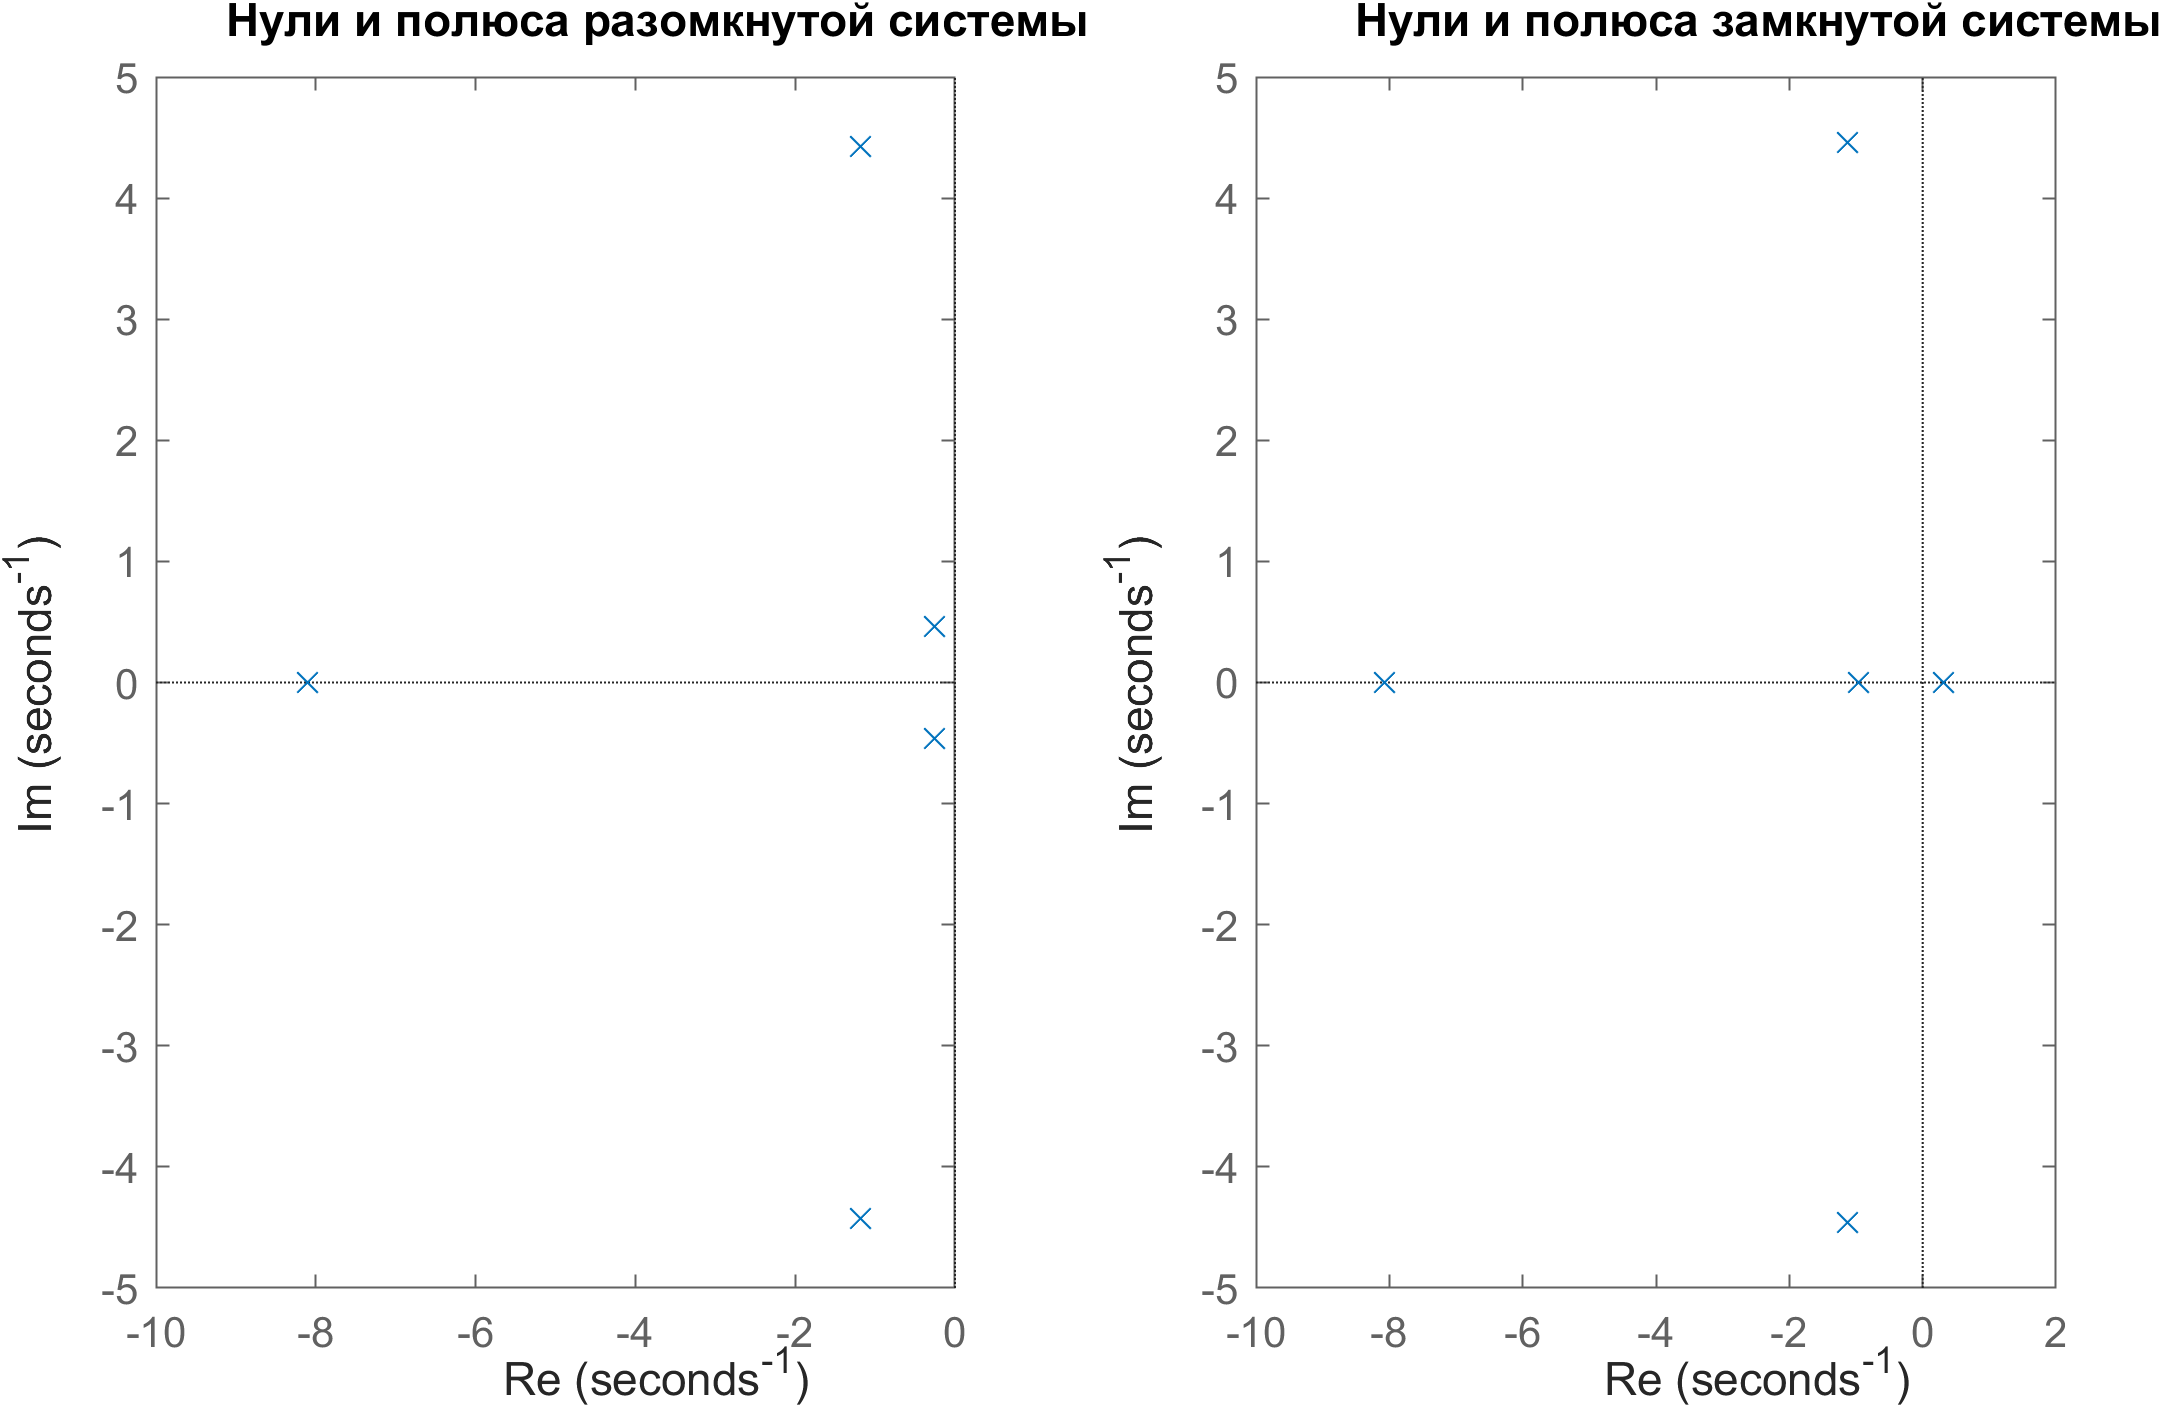
\includegraphics[width=\textwidth]{figs/task_1_obj_2_zeros_poles.png}
    \caption{Нули и полюса объекта 2}
    \label{fig:obj2_pz}
\end{figure}

\begin{figure}[H]
    \centering
    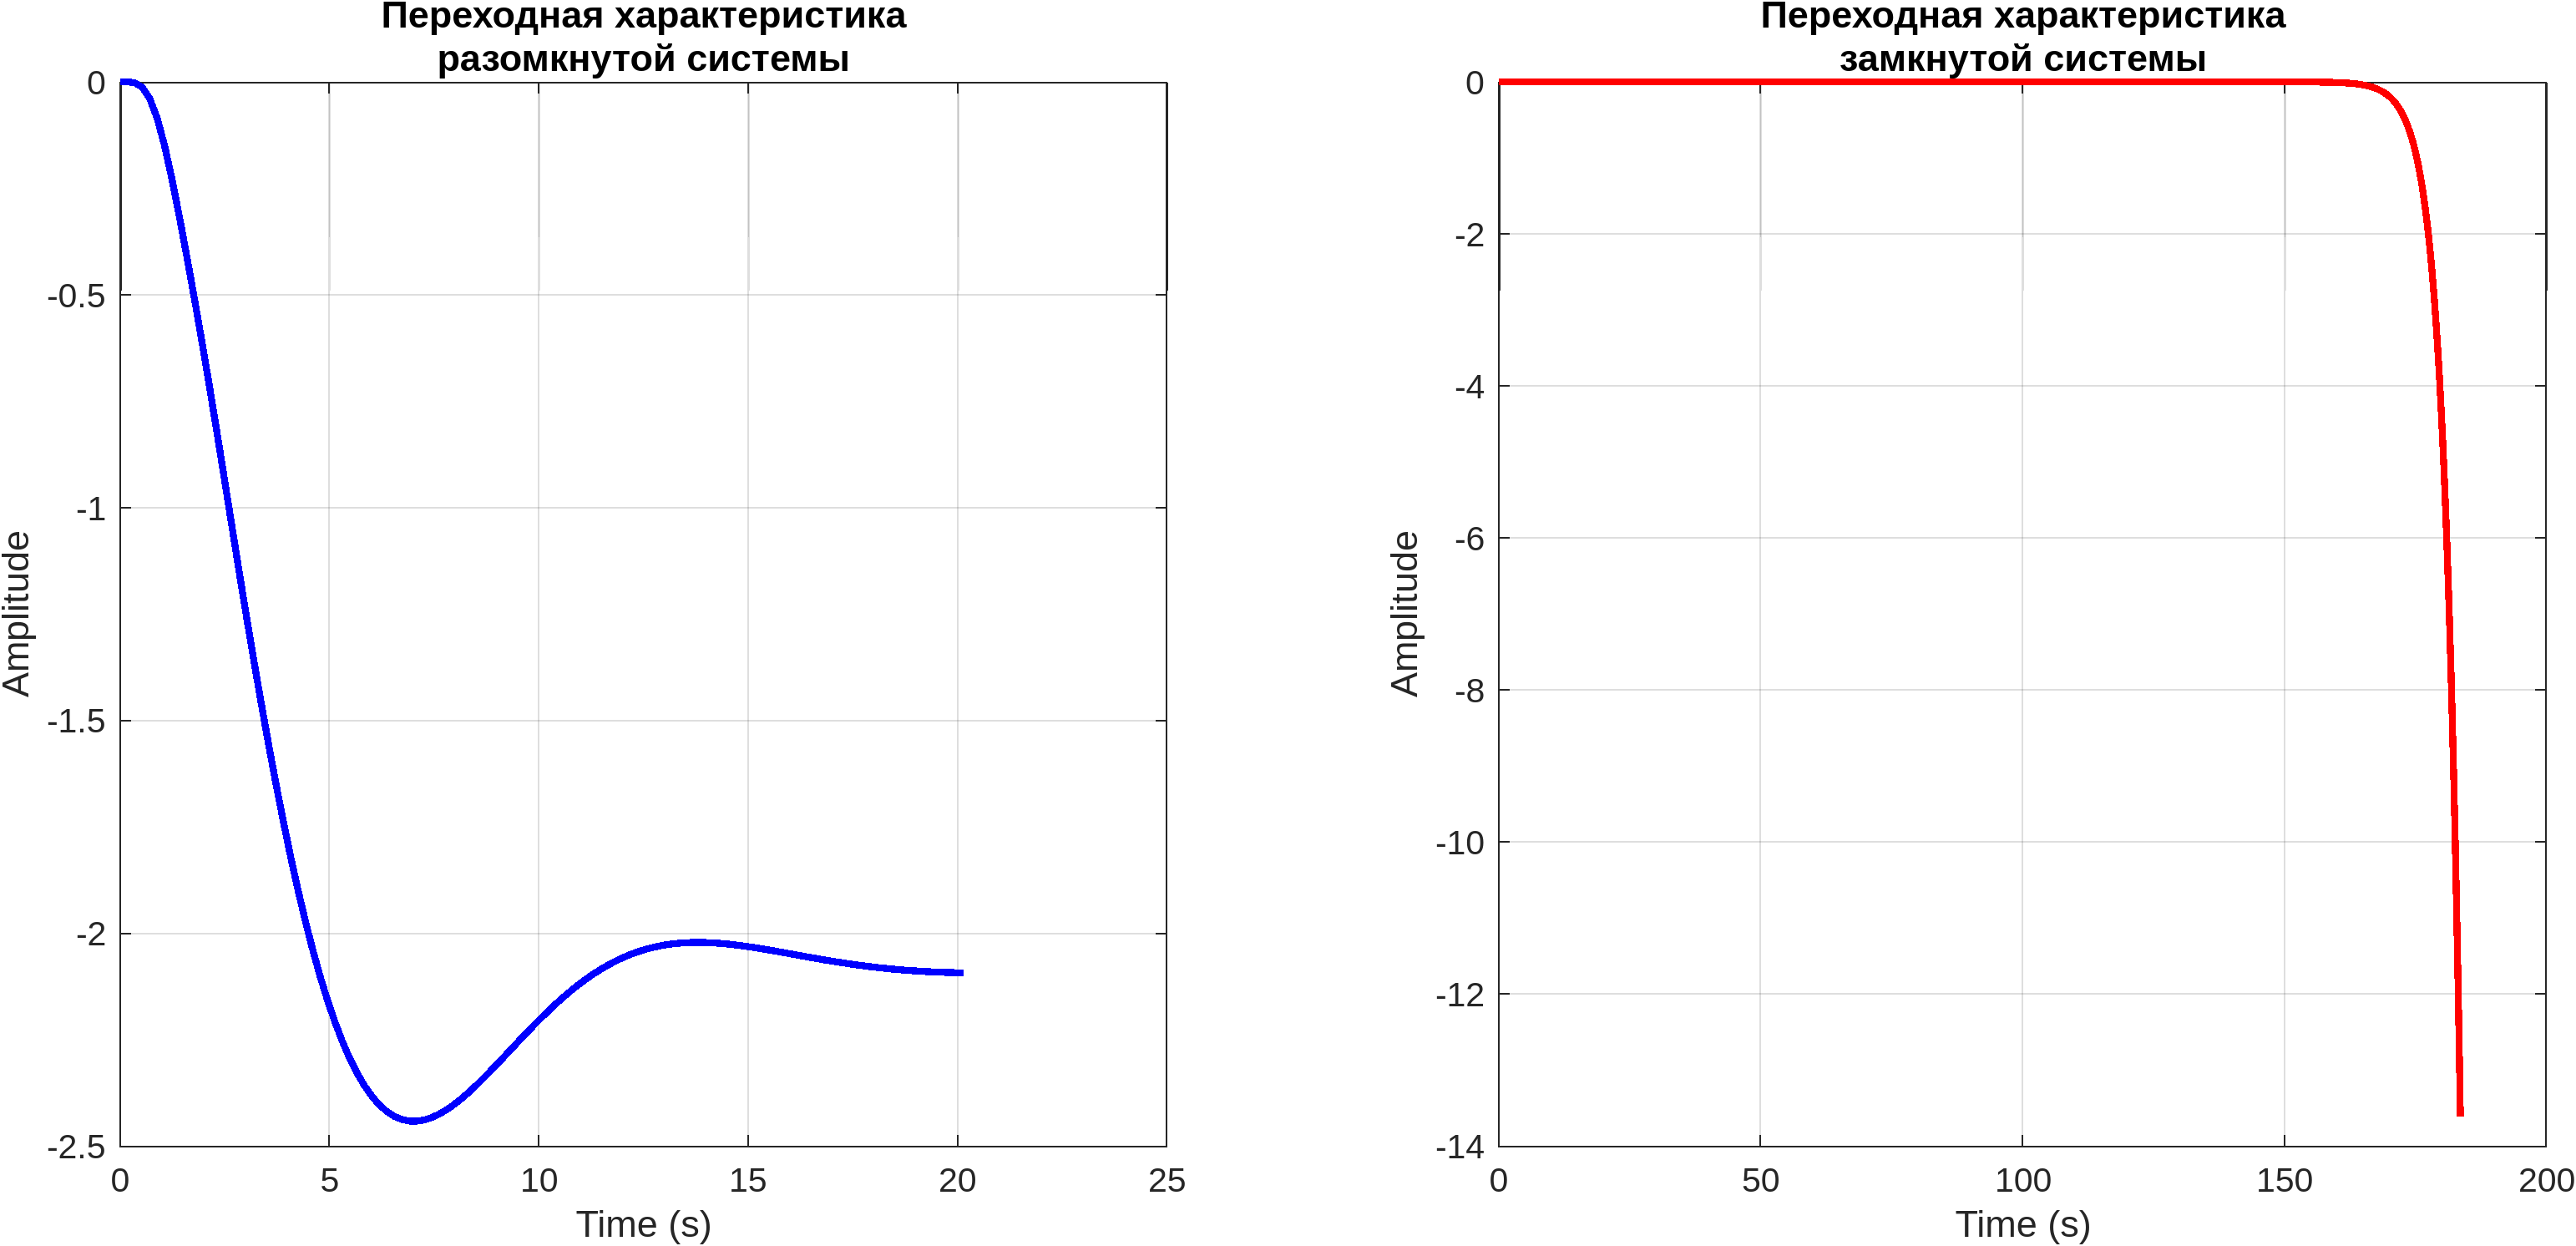
\includegraphics[width=\textwidth]{figs/task_1_obj_2_step.png}
    \caption{Переходные характеристики объекта 2}
    \label{fig:obj2_step}
\end{figure}

\begin{figure}[H]
    \centering
    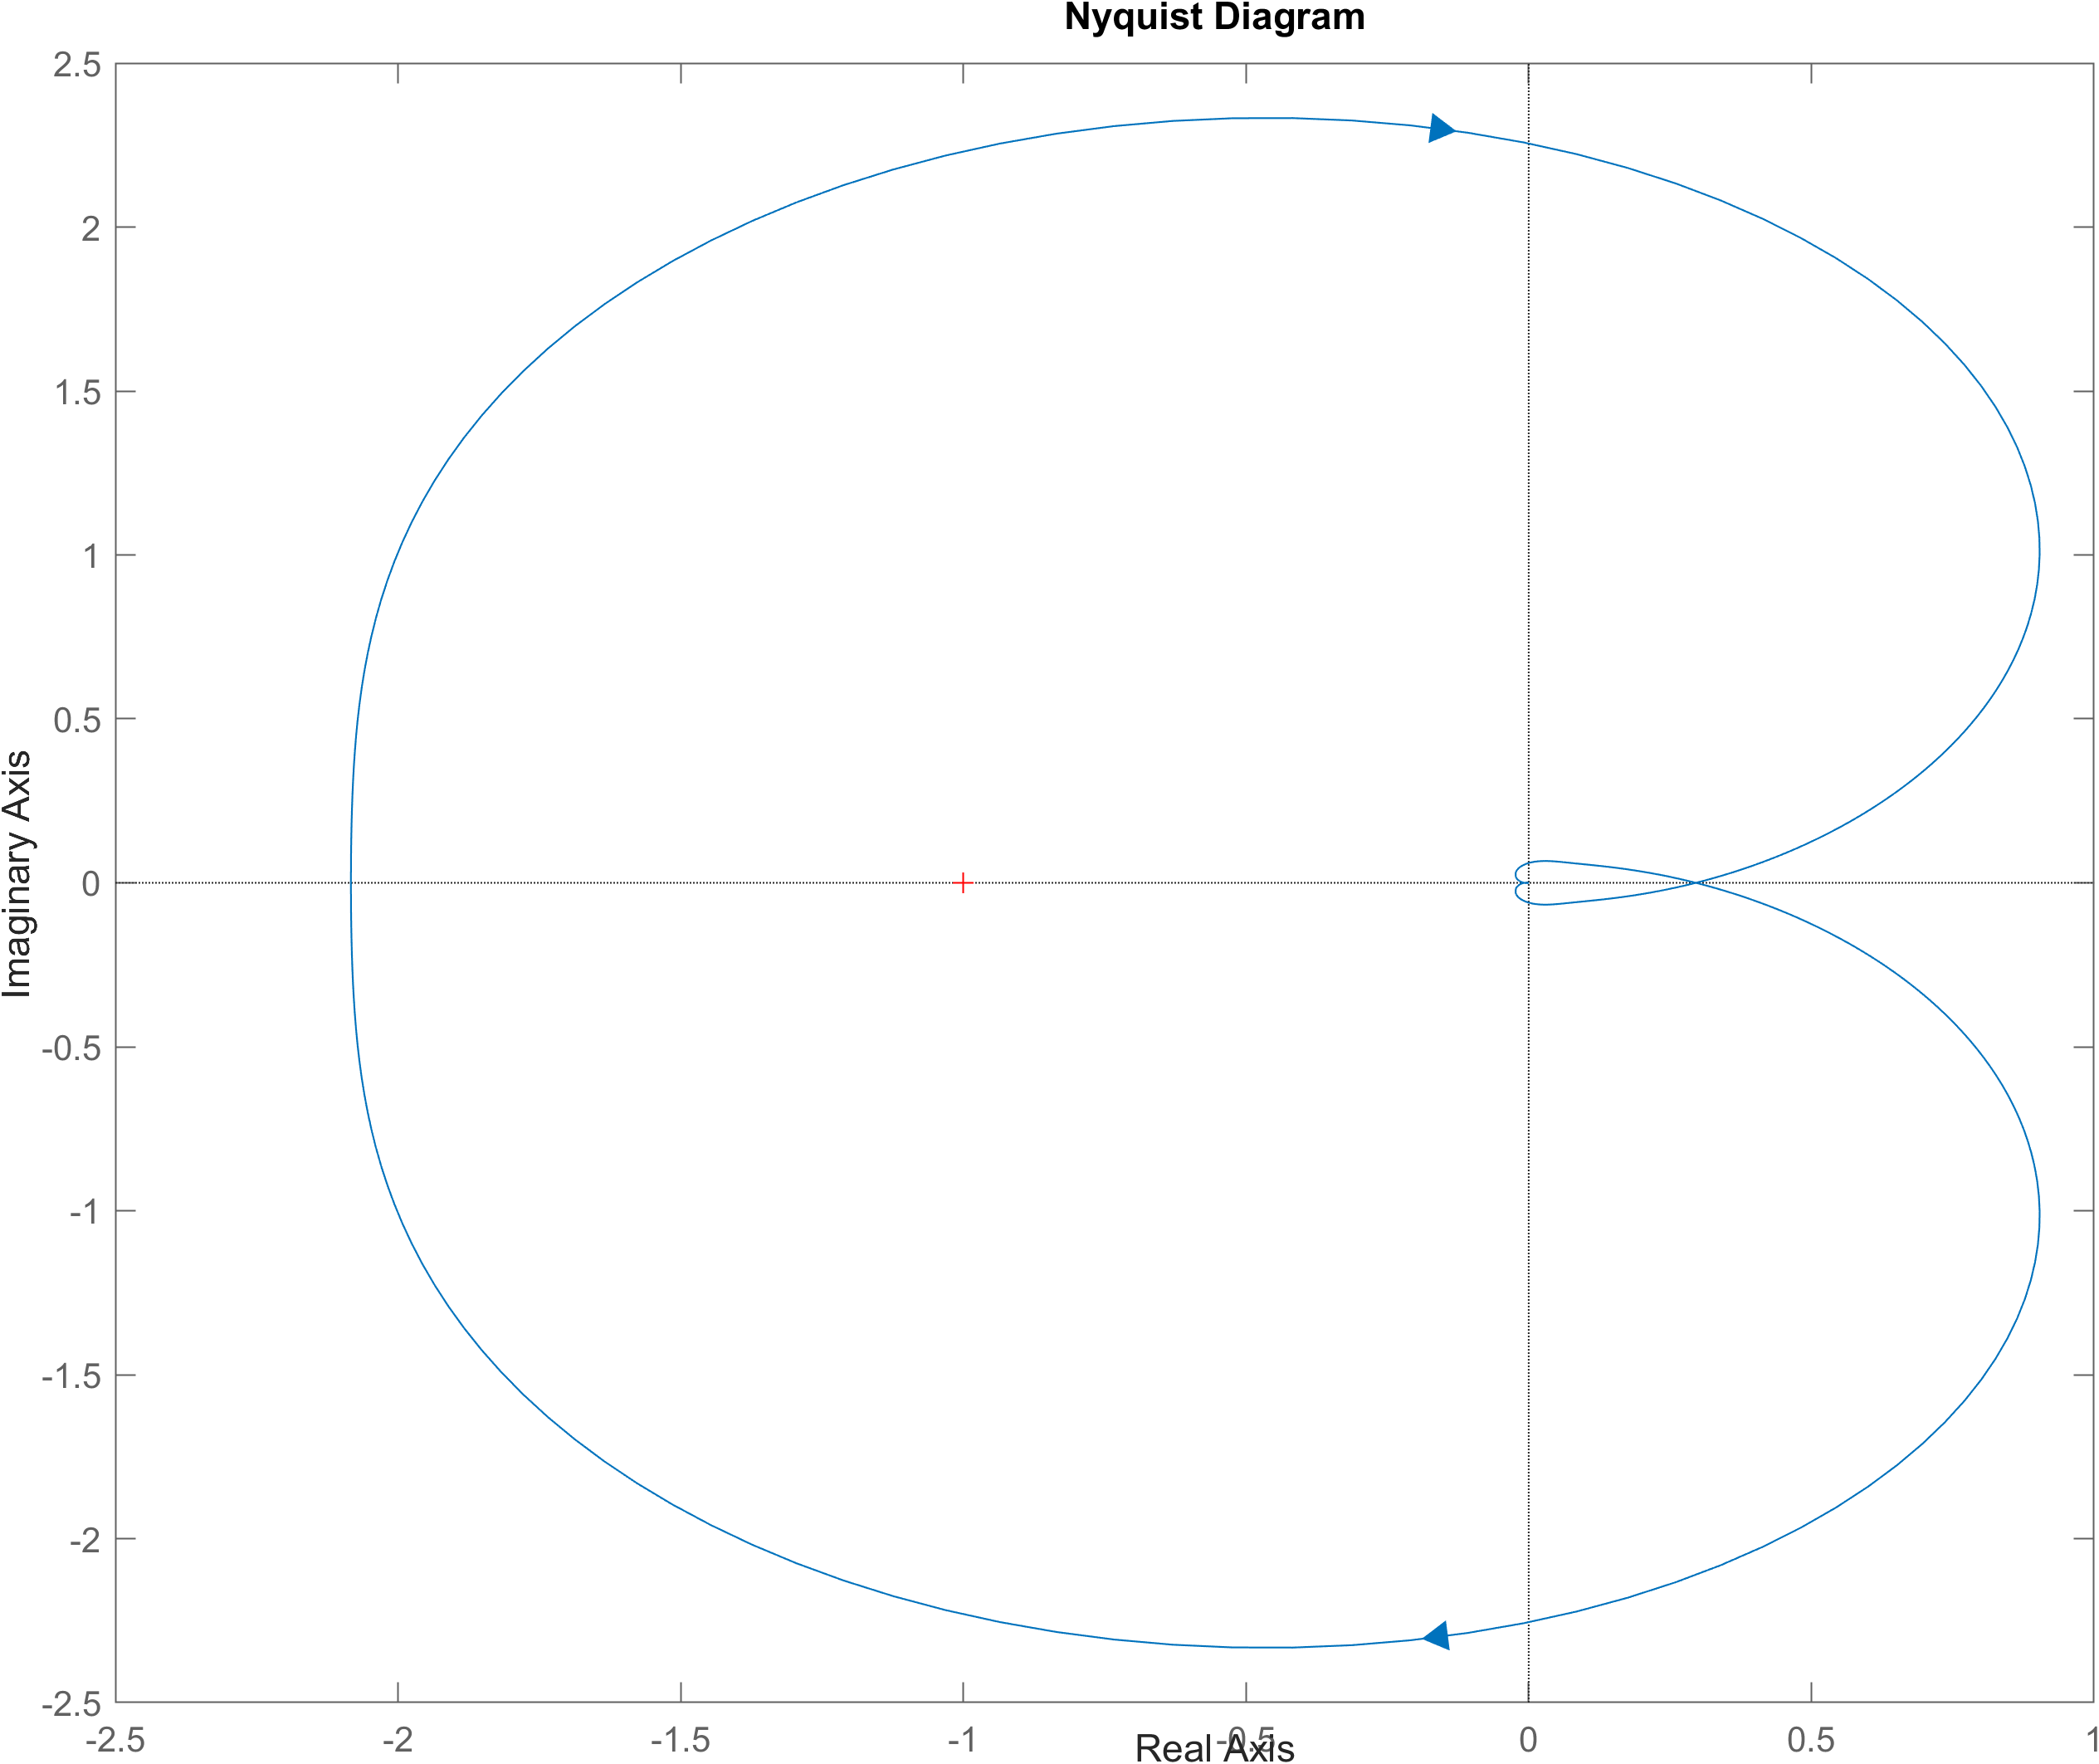
\includegraphics[width=\textwidth]{figs/task_1_obj_2_nyquist.png}
    \caption{Годограф Найквиста объекта 2}
    \label{fig:obj2_nyquist}
\end{figure}

\begin{figure}[H]
    \centering
    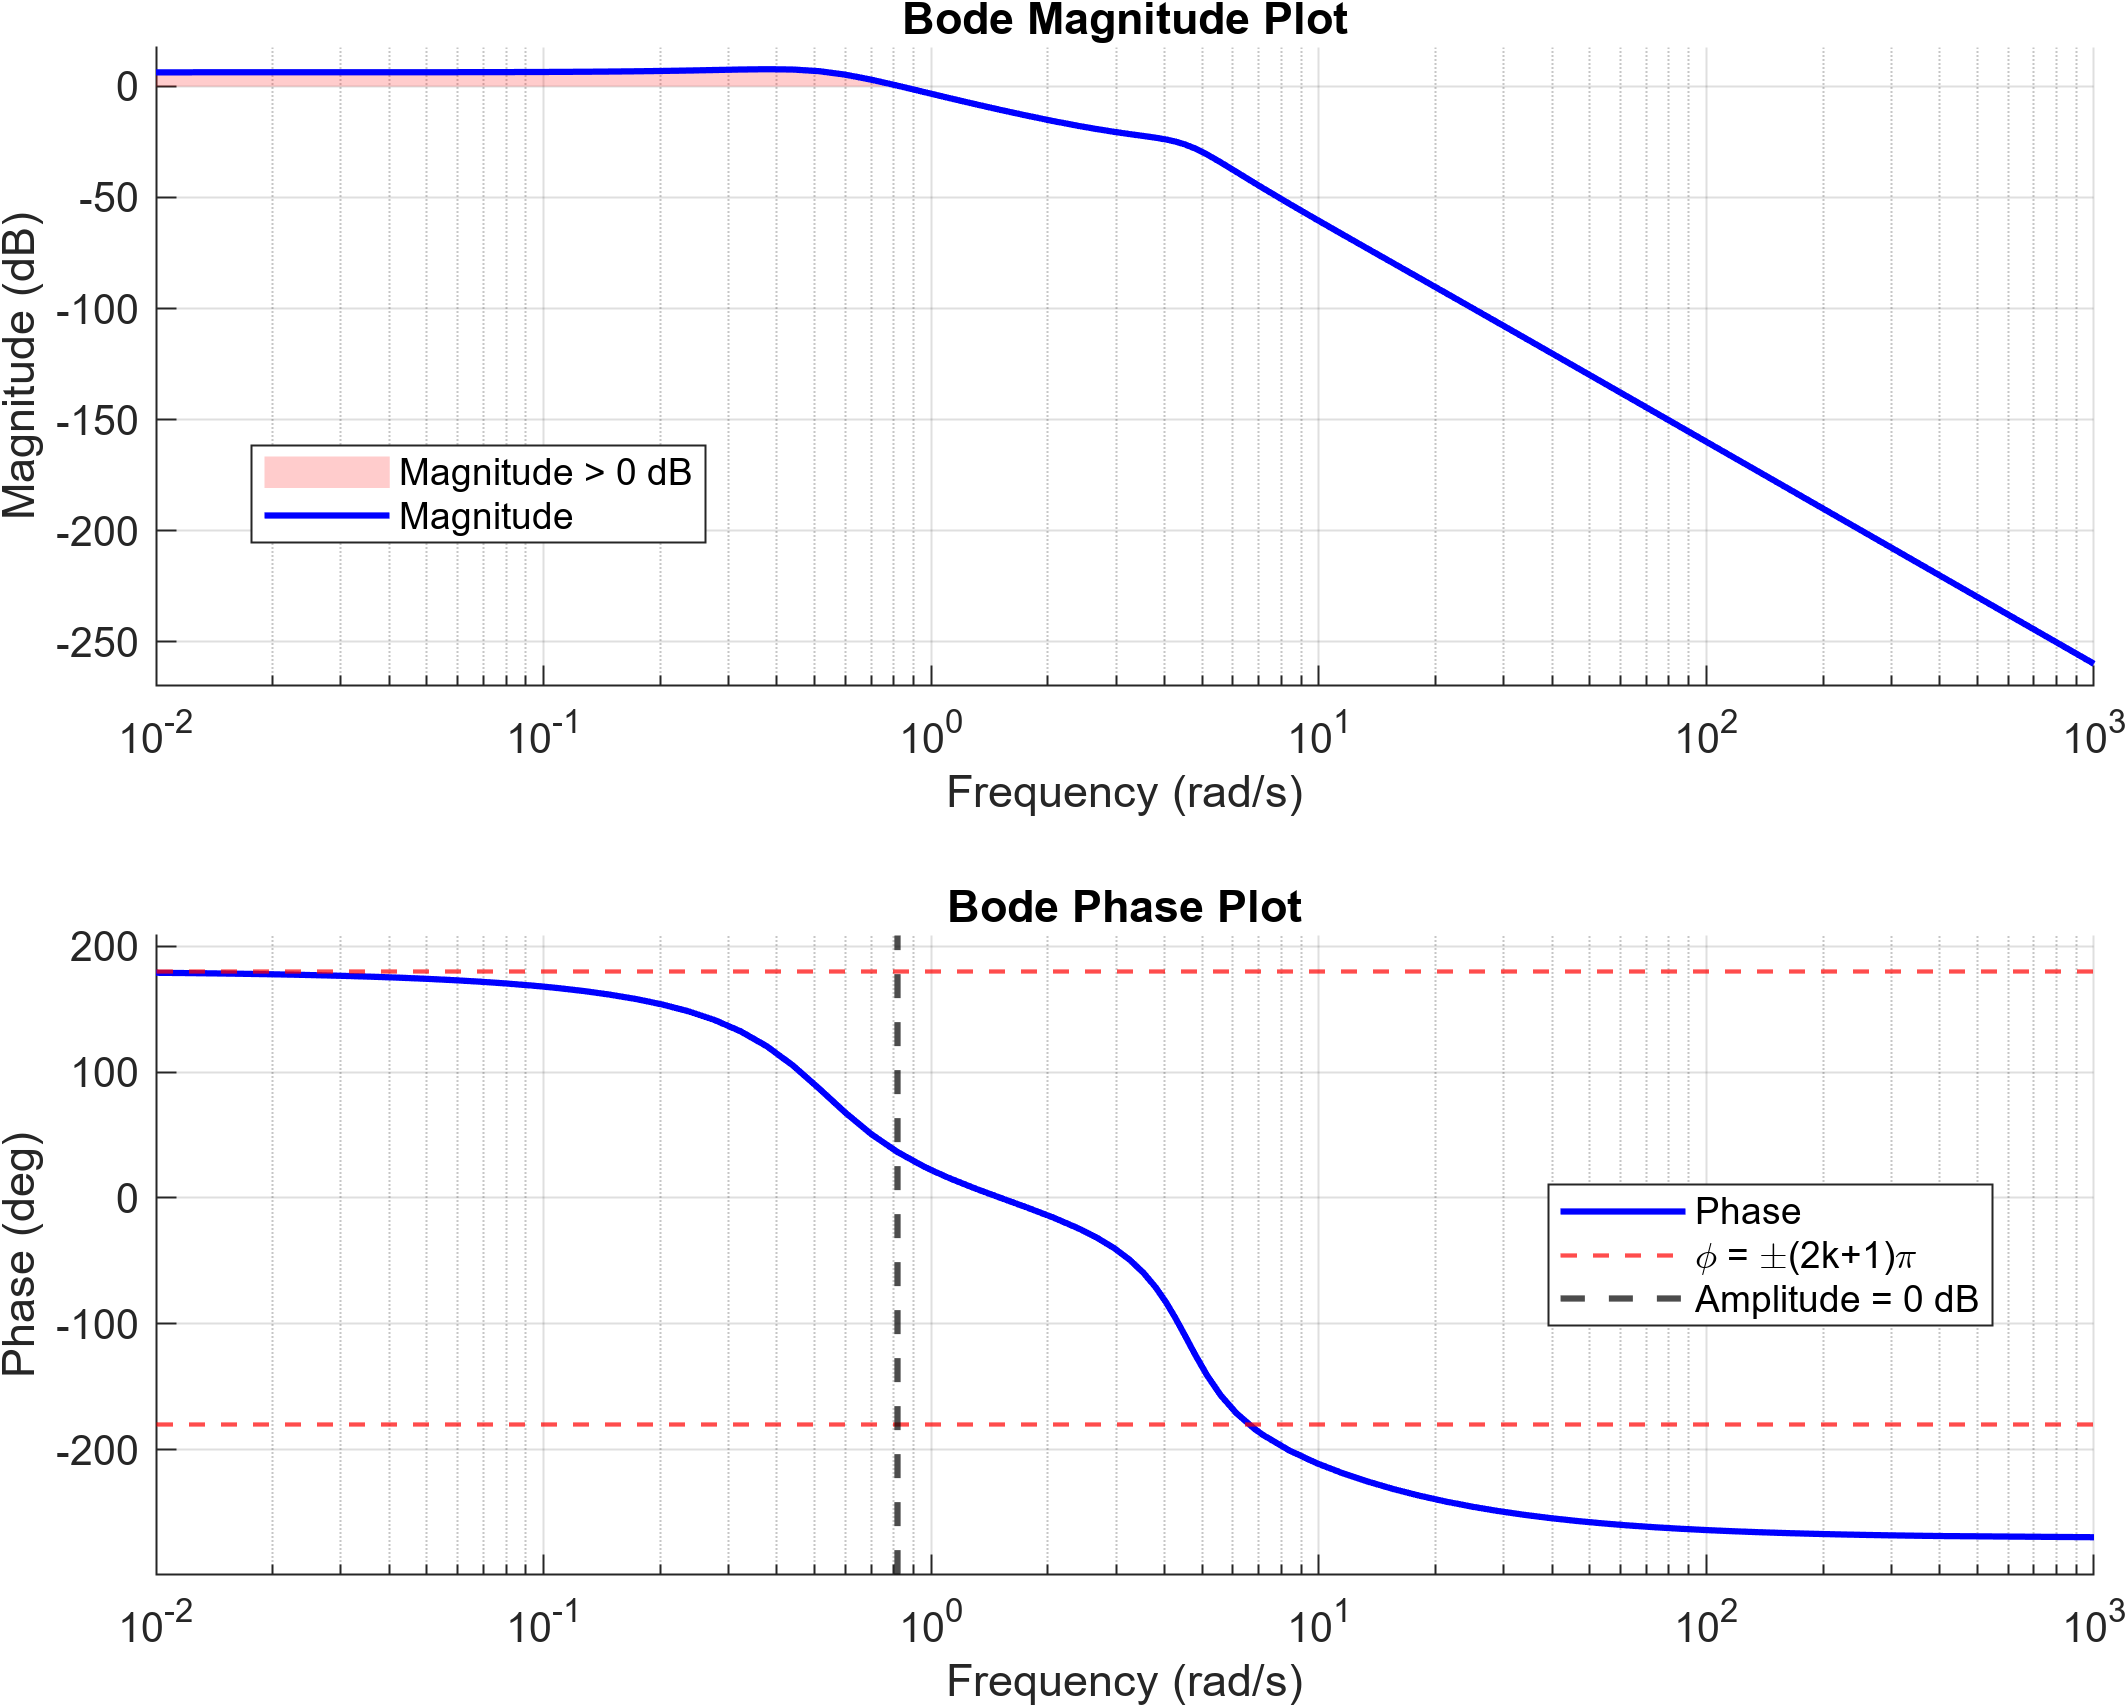
\includegraphics[width=\textwidth]{figs/task_1_obj_2_bode.png}
    \caption{ЛАФЧХ разомкнутой системы объекта 2}
    \label{fig:obj2_bode}
\end{figure}

Переходные характеристики можно увидеть на рисунке \ref{fig:obj2_step},
разомкнутая сходится где-то около -2, а замкнутая расходятся. 
Годограф Найквиста можно увидеть на рисунке 
\ref{fig:obj2_nyquist}, как видно, число оборотов по часовой стрелки
вокруг (-1; 0) равняется 1, что соответствует выводам по критерию Найквиста
выше. ЛАФЧХ разомкнутой системы можно увидеть на рисунке \ref{fig:obj2_bode},
воспользовавшись логарифмическим критерием Найквиста, убеждаемся, что 
замкнутая система не будет устойчива, так как переходов $-\frac{1}{2}$, а нужно $0$.


\newpage
\subsection{Объект 3}

ПФ с четырьмя неустойчивыми полюсами у разомкнутой системы и без таковых у замкнутой,
разомкнутая система:
\begin{equation*}
    W_3(s)=\frac{s^5+31s^4+330s^3+1300s^2+1000s}{(s-1-j)(s-1+j)(s-2)(s-3)(s+1)}
    = \frac{s^5+31s^4+330s^3+1300s^2+1000s}{s^5-6s^4+11s^3-4s^2-10s+12}.
\end{equation*}

Полюса разомкнутой и замкнутой систем можно увидеть в таблице \ref{tab:poles3},
как и их изображение на комплексной плоскости на рисунке \ref{fig:obj3_pz}
вместе с нулями. Было три неустойчивых корня, стало 0, значит по критерию 
Найквиста разность между оборотами АФЧХ вокруг (-1; 0) по часовой стрелки и против часовой стрелке
равняется 4.

\begin{table}[H]
    \centering
    \caption{Полюса объекта 3}
    \begin{tabular}{|c|c|}
    \hline
    \textbf{Полюса разомкнутой системы}       & \textbf{Полюса замкнутой системы}        \\ \hline
        $3.0000 + 0.0000i$ & $-3.8683 + 10.7179i$ \\ \hline
        $-1.0000 + 0.0000i$ & $-3.8683 - 10.7179i$ \\ \hline
        $2.0000 + 0.0000i$ & $-3.7512 + 0.0000i$ \\ \hline
        $1.0000 + 1.0000i$ & $-1.0000 + 0.0000i$ \\ \hline
        $1.0000 - 1.0000i$ & $-0.0123 + 0.0000i$ \\ \hline
    \end{tabular}
    \label{tab:poles3}
\end{table}

\begin{figure}[H]
    \centering
    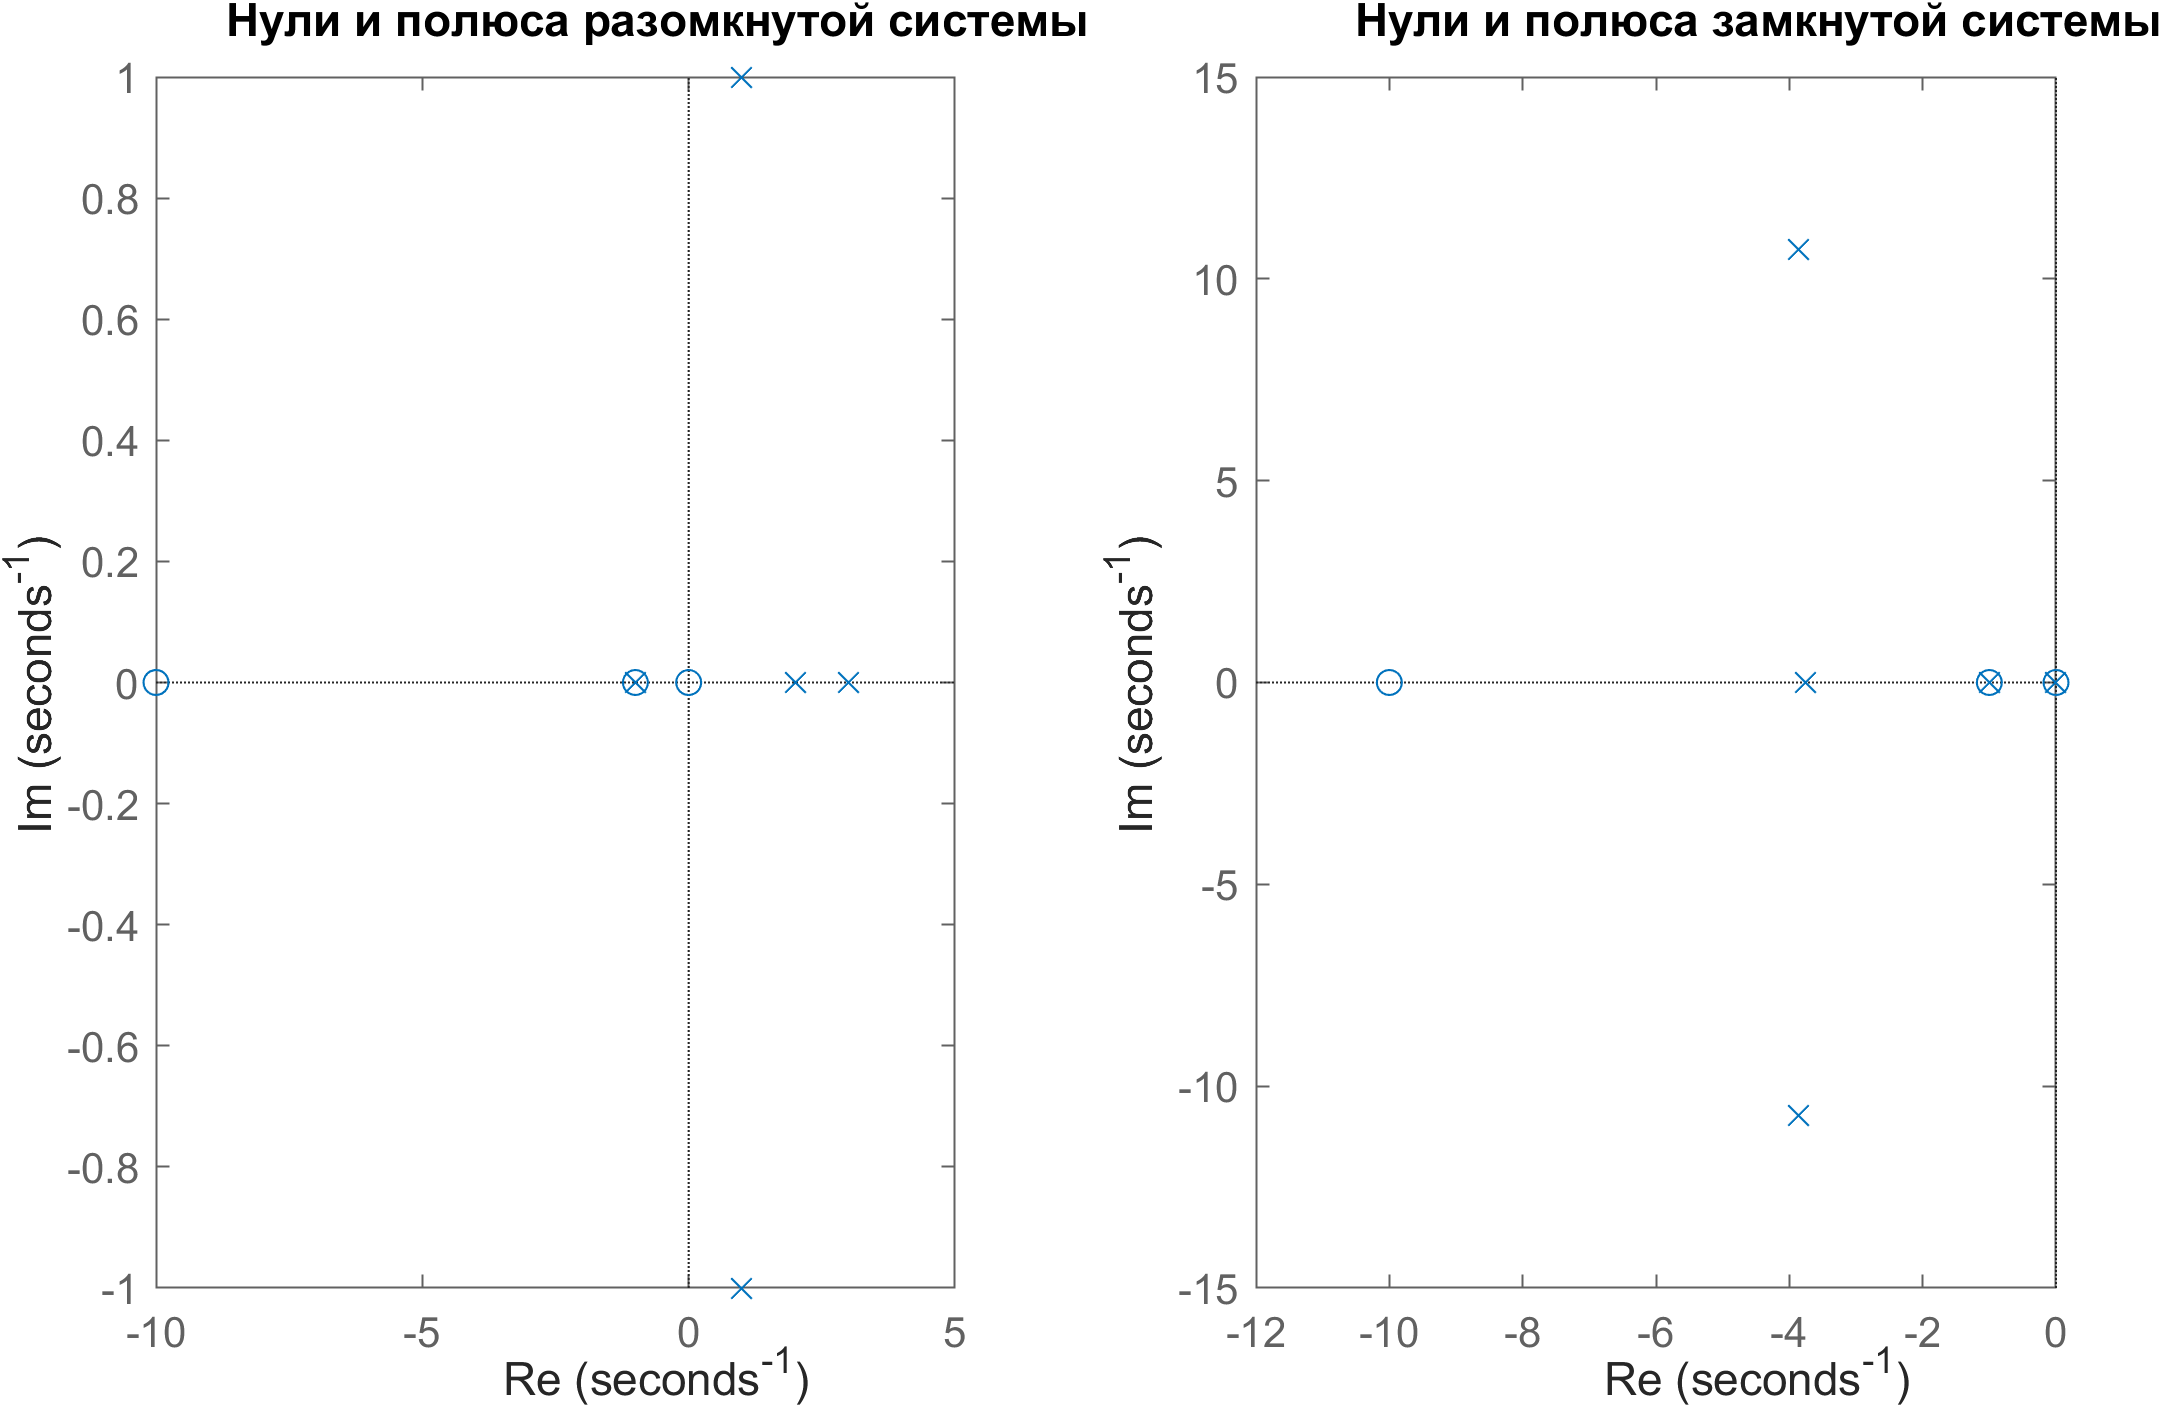
\includegraphics[width=\textwidth]{figs/task_1_obj_3_zeros_poles.png}
    \caption{Нули и полюса объекта 3}
    \label{fig:obj3_pz}
\end{figure}

\begin{figure}[H]
    \centering
    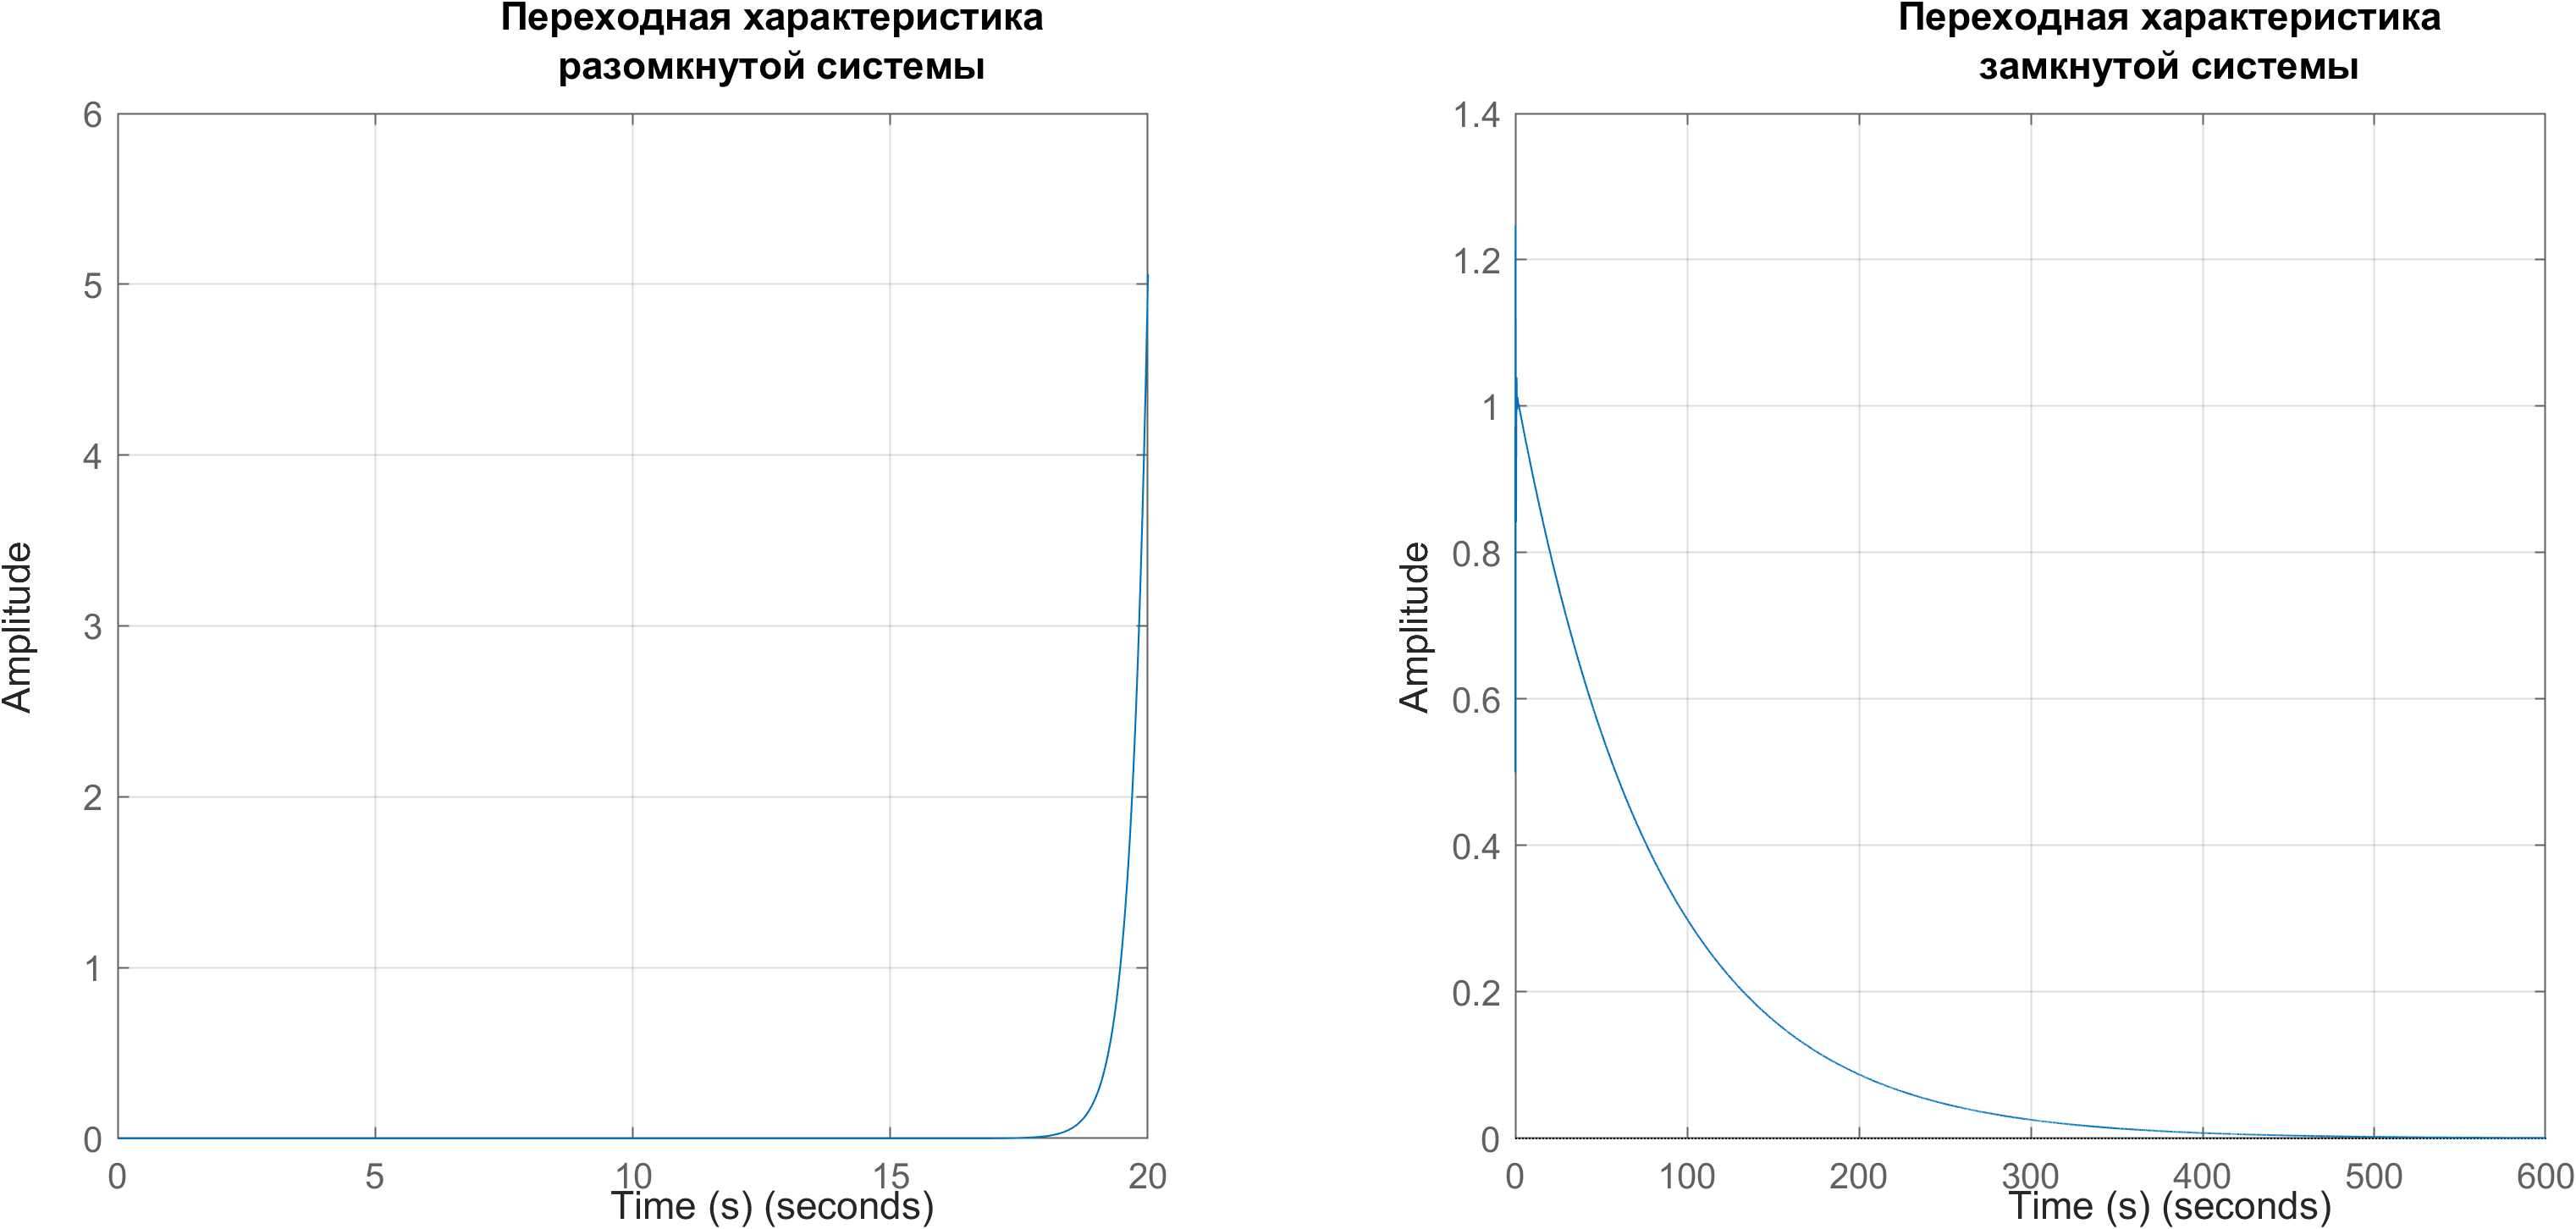
\includegraphics[width=\textwidth]{figs/task_1_obj_3_step.png}
    \caption{Переходные характеристики объекта 3}
    \label{fig:obj3_step}
\end{figure}

\begin{figure}[H]
    \centering
    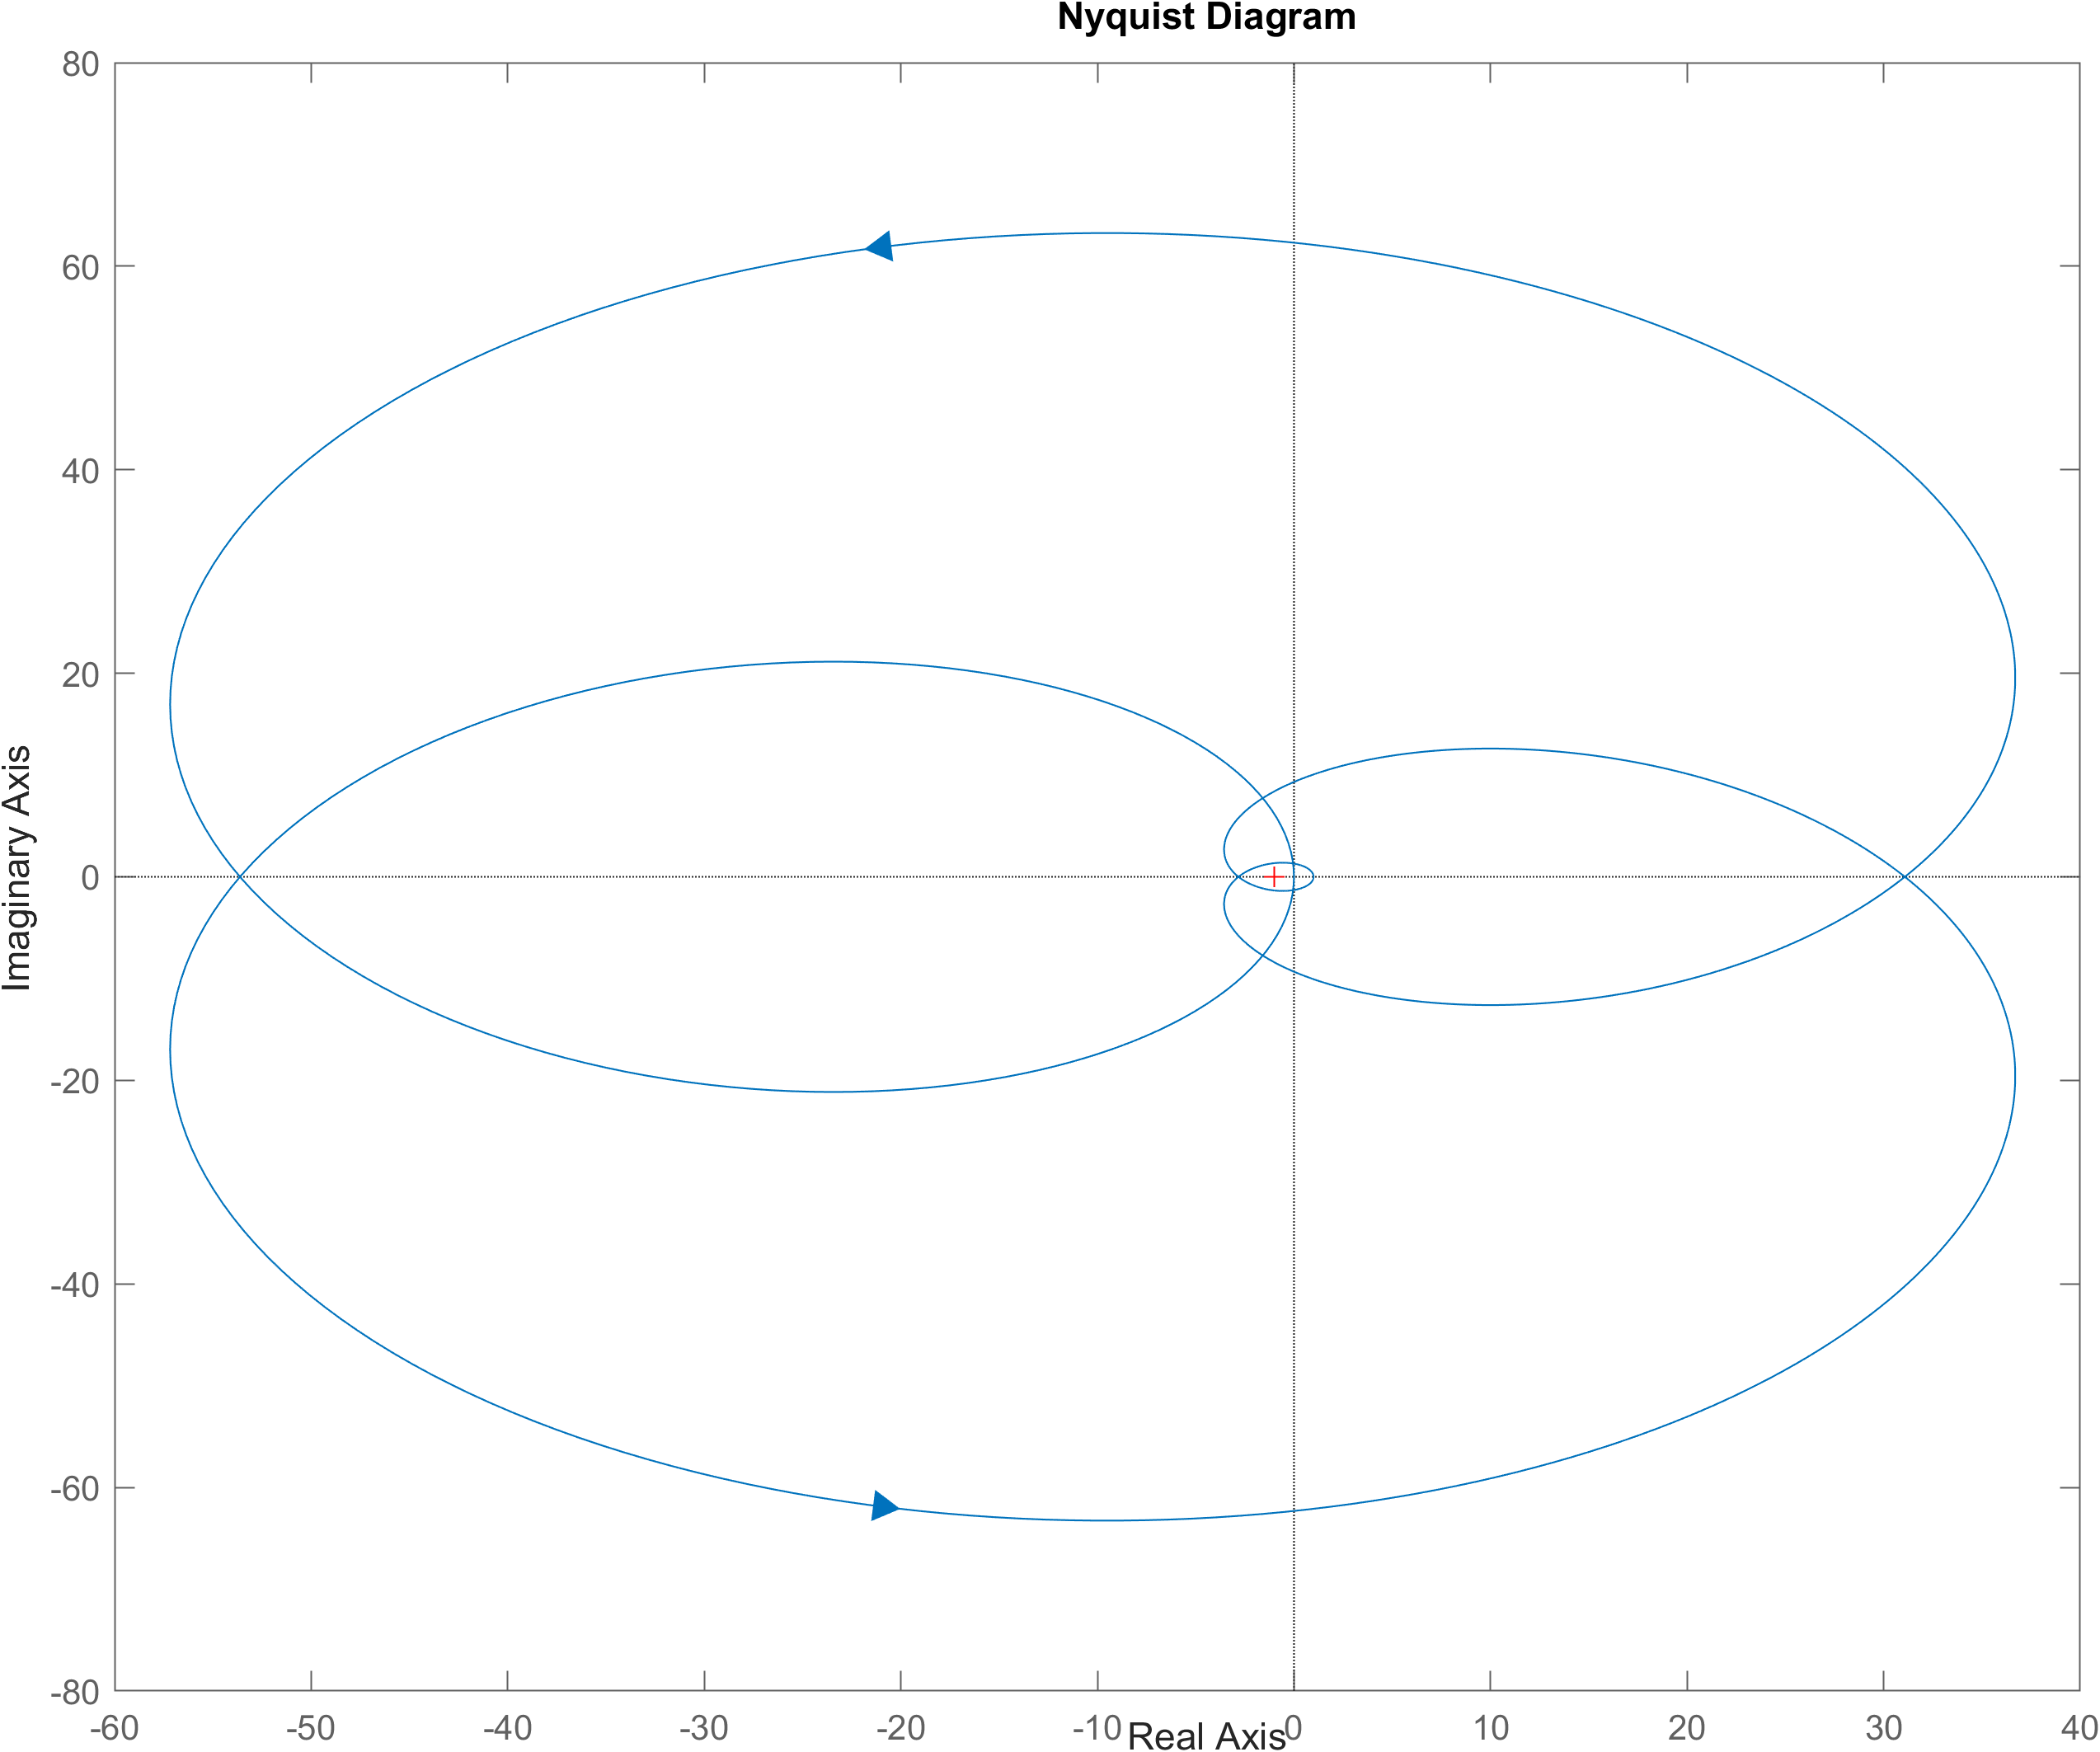
\includegraphics[width=\textwidth]{figs/task_1_obj_3_nyquist.png}
    \caption{Годограф Найквиста объекта 3}
    \label{fig:obj3_nyquist}
\end{figure}

\begin{figure}[H]
    \centering
    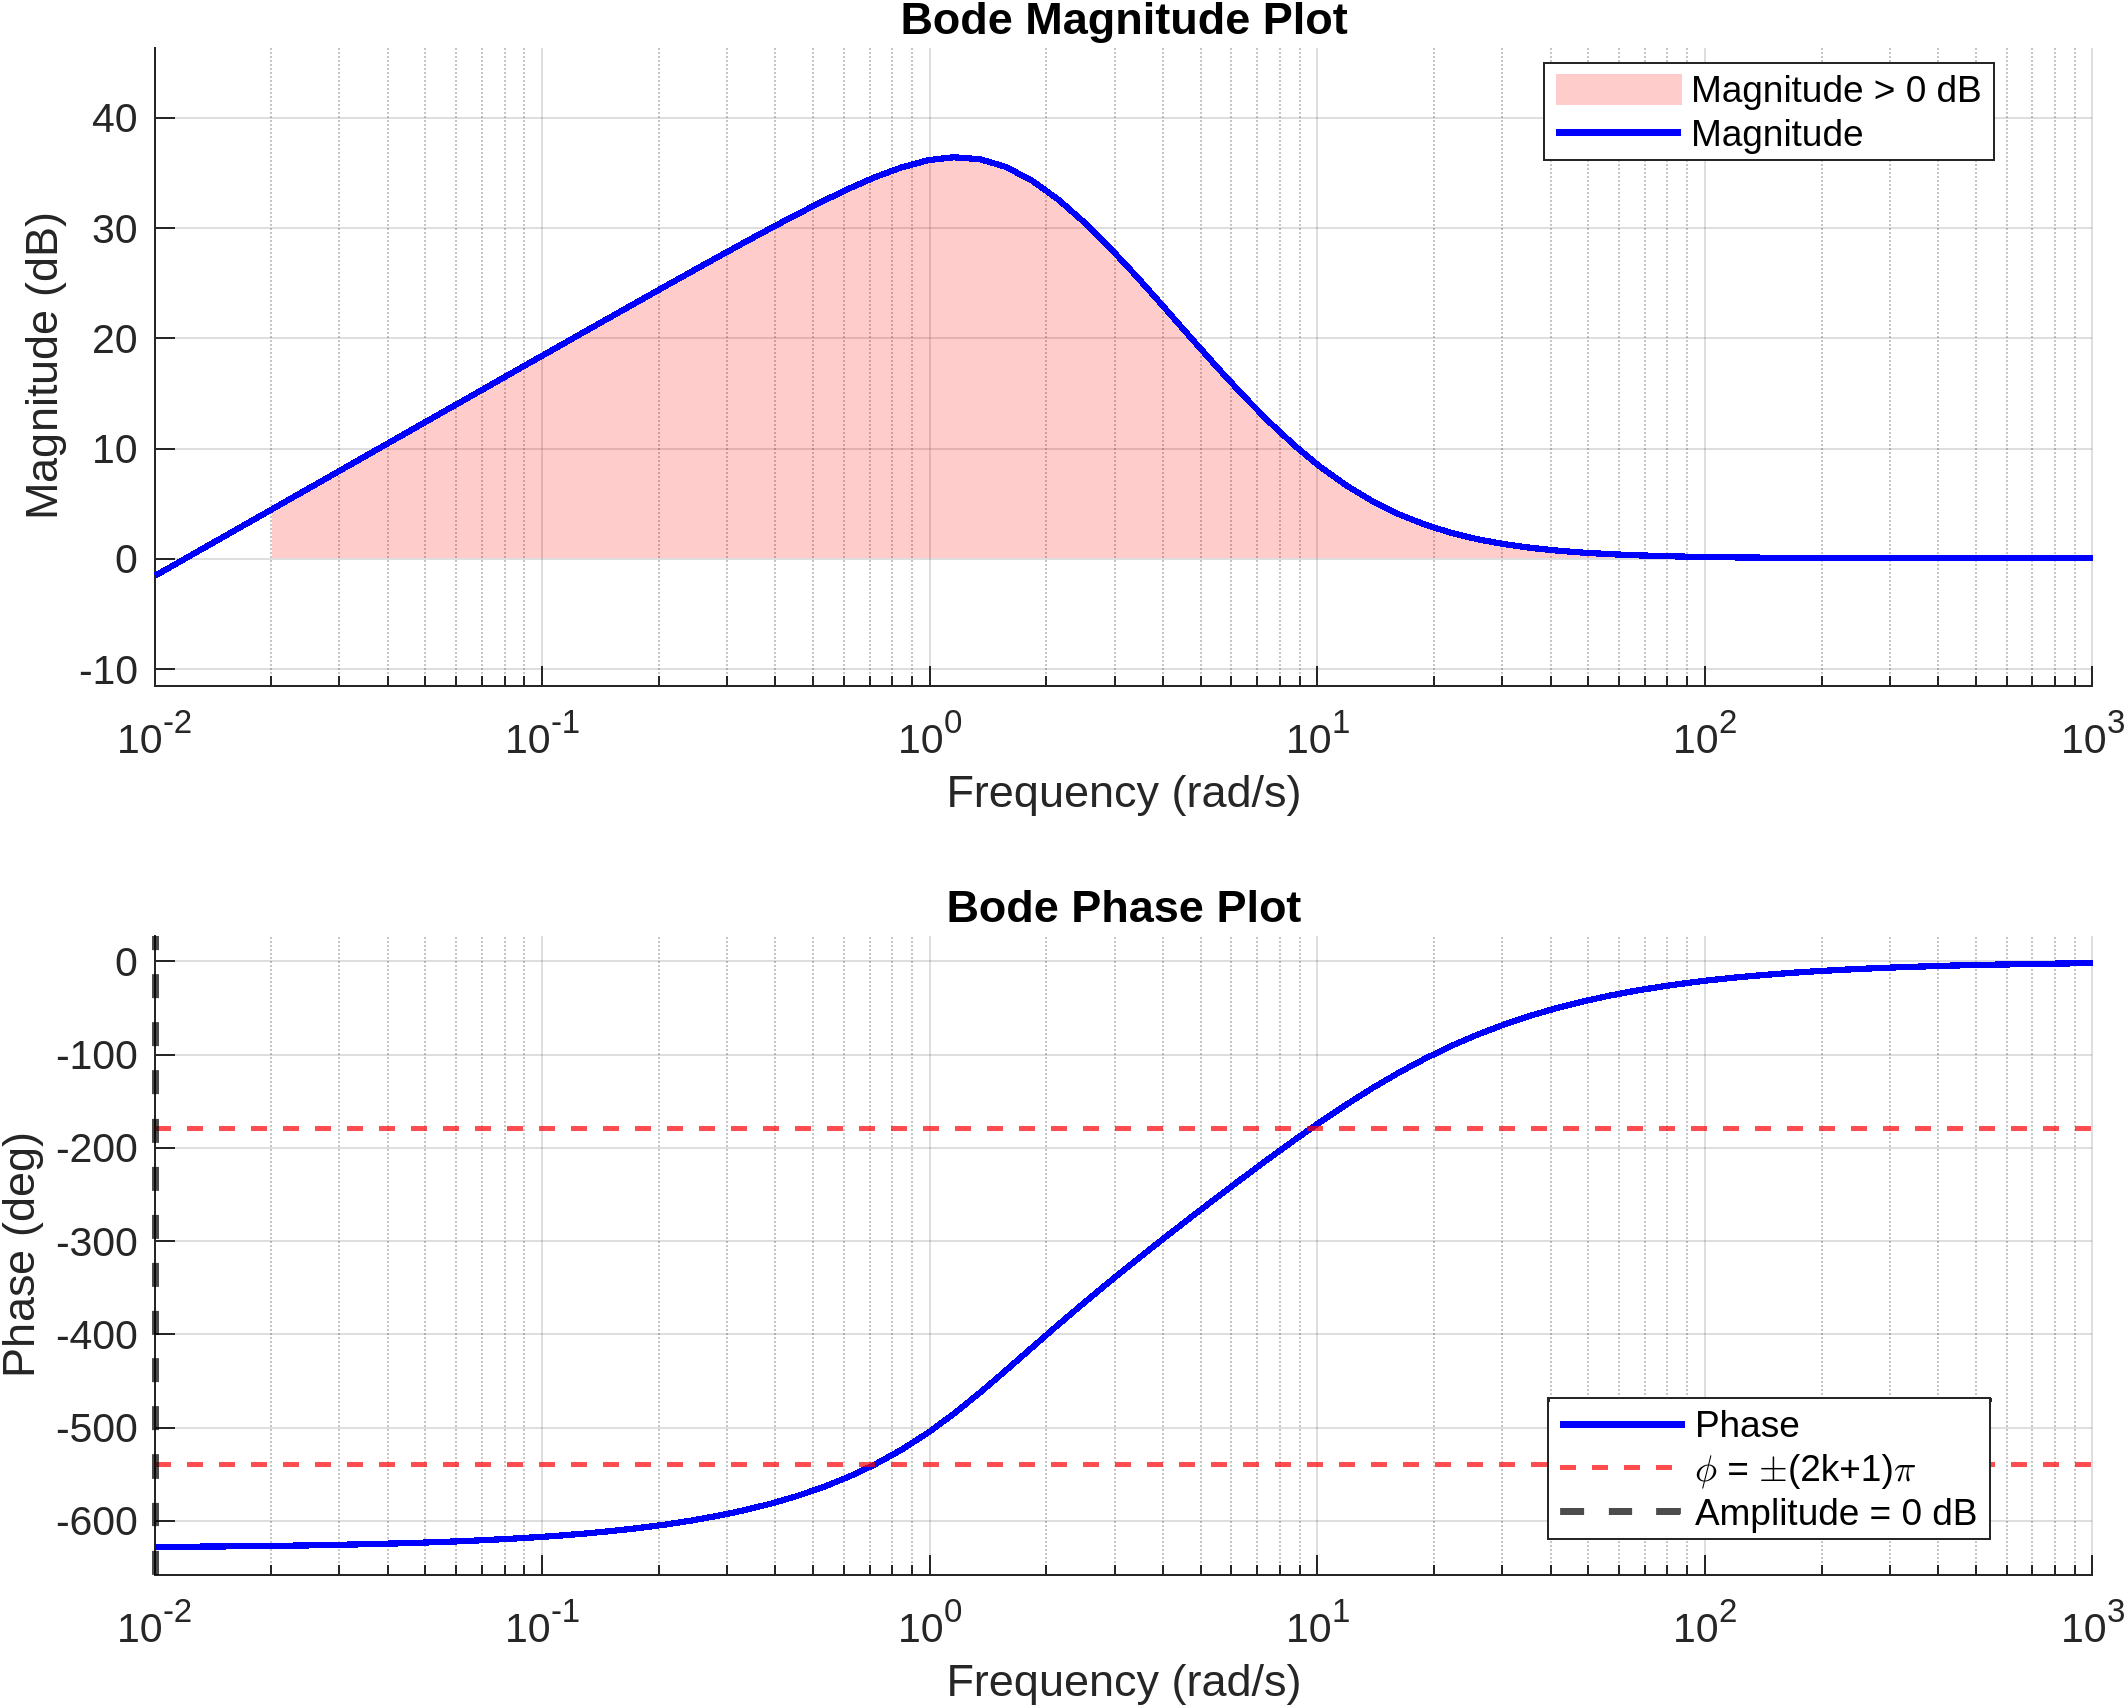
\includegraphics[width=\textwidth]{figs/task_1_obj_3_bode.png}
    \caption{ЛАФЧХ разомкнутой системы объекта 3}
    \label{fig:obj3_bode}
\end{figure}

Переходные характеристики можно увидеть на рисунке \ref{fig:obj3_step},
разомкнутая рассходится, а замкнутая асимптотичесхи сходится. 
Годограф Найквиста можно увидеть на рисунке 
\ref{fig:obj3_nyquist}, как видно, число оборотов против часовой стрелки
вокруг (-1; 0) равняется 4, что соответствует выводам по критерию Найквиста
выше. ЛАФЧХ разомкнутой системы можно увидеть на рисунке \ref{fig:obj3_bode},
воспользовавшись логарифмическим критерием Найквиста, убеждаемся, что 
замкнутая система будет устойчива, так как переходов $2$, и нужно $2$.


\section{Коэффициент усиления}

